\documentclass[11pt]{article}
\usepackage[small]{titlesec}
\usepackage[top = 0.66in,textwidth = 6.5in, textheight=9.1in]{geometry}

\usepackage{amsmath}
\usepackage{scalefnt}
\usepackage{graphicx}
\usepackage{latexsym}
\usepackage{color}
\usepackage{amssymb}
\usepackage{accents}
\usepackage{tabularx}
\usepackage{fancyhdr}
\usepackage{verbatim}
\usepackage{multirow}
\usepackage{framed}
\usepackage[square,sort,comma,numbers]{natbib}
\bibpunct[, ]{(}{)}{,}{a}{}{,}%
	\def\bibhang{24pt}%
	\def\newblock{\ }%
	\def\BIBand{and}
\usepackage{url}
\usepackage{float, subfig}
\usepackage{enumitem}
\usepackage{mathtools}
\usepackage{mathrsfs}
\usepackage{amsfonts}
\usepackage{listings}
\usepackage{amsthm}
\usepackage{grffile}
\usepackage{sidecap}
\usepackage{pbox}
\usepackage{algorithm}
\usepackage{longtable}
\usepackage[noend]{algpseudocode}

\def\qed{\hfill{\(\vcenter{\hrule height1pt \hbox{\vrule width1pt height5pt
     \kern5pt \vrule width1pt} \hrule height1pt}\)} \medskip}

\newtheorem{theorem}{Theorem}
\newtheorem{lemma}[theorem]{Lemma}
\newtheorem{corollary}[theorem]{Corollary}
\newtheorem{proposition}[theorem]{Proposition}
\newtheorem{assumption}{Assumption}
\newtheorem{conjecture}[theorem]{Conjecture}
\newtheorem{remark}{Remark}
\newtheorem{example}{Example}
\newtheorem{definition}{Definition}
\renewcommand{\textfraction}{0.0}
\newcommand{\dst}{\displaystyle}
\newcommand{\minx}{\mbox{\( \dst \min_{x \in X} \)}}
\newcommand{\Efx}{\mbox{\( \dst E f (x, \xi) \)}}
\newcommand{\Efxhat}{\mbox{\( \dst E f (\hat{x}, \xi) \)}}
\newcommand{\hxx}{\mbox{\( \hat{x} \)}}
\newcommand{\bpi}{\bar{\pi}}
\newcommand{\xx}{\mbox{\( x \)}}
\newcommand{\txxi}{\mbox{\(\xi\)}}
\newcommand{\var}{\mbox{var}}
\newcommand{\cF}{{\cal F}}
\newcommand{\cA}{{\cal A}}
\newcommand{\cG}{{\cal G}}
\newcommand{\cN}{{\cal N}}
\newcommand{\cQ}{{\cal Q}}
\newcommand{\txi}{{\xi}}
\newcommand{\PP}{\mbox{\(SP\)}}
\newcommand{\PPn}{\mbox{\(SP_n\)}}
\newcommand{\PPnx}{\mbox{\(SP_{n_x}\)}}
\newcommand{\noi}{\noindent}
\renewcommand{\ss}{\smallskip}
\newcommand{\ms}{\medskip}
\newcommand{\bs}{\bigskip}
\newcommand{\st}{\mbox{s.t.}}
\newcommand{\wpo}{\mbox{wp1}}
\newcommand{\iid}{\mbox{i.i.d.\ }}
\newcommand{\vsmo}{\vspace*{-0.1in}}
\newcommand{\vsmt}{\vspace*{-0.2in}}
\newcommand{\vso}{\vspace*{0.1in}}
\newcommand{\vst}{\vspace*{0.2in}}
\newcommand{\mc}{\multicolumn}
\newcommand{\cP}{{\cal P}}
\newcommand{\cH}{{\cal H}}
\newcommand{\thead}{\multicolumn{1}{c |}}
\newcommand{\underv}{\mbox{$\underbar{$v$}$}}
\allowdisplaybreaks 

\renewcommand{\P}{{\mathbb P}}
\newcommand{\E}{{\mathbb E}}
\newcommand{\R}{{\mathbb R}}
\renewcommand{\Re}{{\mathbb R}}
\newcommand{\mbf}{\mathbf}
\renewcommand{\underbar}{\underaccent{\bar}}
\newcommand{\tcr}{\textcolor{red}}
\newcommand{\tcb}{\textcolor{blue}}

\begin{document}
%0.27
\baselineskip0.25in

\begin{center}
\begin{large}
\begin{bf}

Optimal Crashing of an Activity Network with Disruptions \ms

\today \ms
\end{bf}
\end{large}
\end{center}

\section{Introduction} \label{sec:introduction}
	The management of complex projects through optimization has a rich history in operations research, beginning with the critical path method of \cite{kelley1961criticalpath}; see \citet{soderlund2004building} for an overview. A project is a collection of activities, between which there are precedence relationships due to logical or technological considerations. A precedence relationship is usually reflected as the start time of one activity following the completion of another. 
	%a required separation time between the start time of two activities. 
	Typically, multiple activities can be processed at the same time, and there is no limit on how many activities can be processed simultaneously, as long as the precedence requirements are satisfied. See~\citet{Elmaghraby77} for a detailed treatment of activity networks. In this setting, ``crashing" is an action that consumes a certain amount of one or more resources and shortens the duration of an activity accordingly~\citep{kuhl2008dynamic}. A deterministic optimization model for crashing an activity network was proposed in the 1960s \citep{fulkerson1961network, kelley1961criticalpath}, in which the goal is to complete the project in minimum time by allocating resources under one or more budget constraints.
	
	When the program evaluation and review technique (PERT) was introduced~\citep{malcolm1959application}, activity durations were modeled as independent beta random variables, and the project duration approximated by a normal distribution. Extensions that allow for more general assumptions followed \citep{Elmaghraby77}, and Monte Carlo simulation plays a role in estimating the expected project span, which is difficult to express analytically \citep{burt1971conditional,van1963letter}.
	Heuristics and simulation-based algorithms have been developed to approximately solve the stochastic project crashing problem \citep{aghaie2009ant, bowman1994stochastic, ke2014genetic, kim2007heuristic}. Another approach to handle uncertainty in activity duration is robust optimization, in which the objective is to minimize the worst case project span over a specified uncertainty set. While affinely adaptive recourse decisions are computationally tractable as linear, or second-order cone, programs, this restriction may lead to suboptimal solutions \citep{chen2008linear, cohen2007stochastic}. However, once recourse decisions can take general form, the robust model is only tractable with rectangular uncertainty sets
	\citep{wiesemann2012robust}. \citet{ahipasaoglu2016distributionally} propose a distributionally robust optimization scheme applied to a PERT network, which reformulates the problem as a semidefinite program or a copositive program, depending on the description of uncertainty. The project crashing optimization problem finds application in project management~\citep{demeulemeester2006project, jaselskis1991allocation,tonchia2018industrial}, machine scheduling~\citep{blazewicz1983scheduling,hall1996machine}, health services scheduling~\citep{cardoen2010operating}, chemical processes~\citep{li2008process}, and digital circuit sizing~\citep{kim2007heuristic}.

	In this paper, we propose using the concept of stochastic disruptions to model uncertainty in the duration of activities, which differs from existing approaches in both stochastic programming and robust optimization. A stochastic disruption is an event that may occur at any point in the problem's time horizon and results in a change---typically a significant change---in the system's parameters. A few authors apply this idea in models with discrete time periods, in which the disruption can only occur in a set of specified time periods. \citet{yu2004disruptionmgt} introduce scenario-based optimization models for airline scheduling. \citet{morton2009sealift} introduce a sealift scheduling problem under a finite number of stochastic disruptions within a stochastic programming structure; this model structure ``falls between standard two-stage and multi-stage stochastic programs for a multi-period problem" and reduces the size of the problem (scenario tree) to quadratic, rather than exponential, growth in the number of time periods. Our setting inherits the philosophy of \citet{morton2009sealift}, but enhances the model by allowing the random disruption time to be continuous in the context of an activity network, instead of a prespecified set of fixed time periods. 

	Given a limited number of disruption scenarios, the problem of optimizing crashing decisions to minimize expected completion time can be formulated as a stochastic mixed-integer program, and we present the model in Section~\ref{sec:formulation}. If we assume a continuous distribution for the disruption time and magnitude, a sample average approximation (SAA) can be used to create a finite set of scenarios and approximate the original problem by a finite-sized optimization problem. In Section~\ref{sec:nphard} we show that the problem is NP-hard even with continuous allocation of crashing effort and just two scenarios. Section~\ref{sec:examples} presents properties of the problem using a serial activity network as a special case. The potentially large scale and the discrete, non-convex nature of the SAA problem's formulation suggest that it may be computationally challenging to solve. In Section~\ref{sec:decomposition}, a method based on Benders' decomposition is developed to solve our problem of optimizing crashing decisions under stochastic disruptions. We show such a decomposition method can solve the integer program in a finite number of iterations. Experiment results are presented in Section~\ref{sec:results}, including the empirical relationship between solution quality and sample size, the comparison between the quality of our solution and solutions of alternative models, and the computational performance of the decomposition method of Section~\ref{sec:decomposition}. We conclude with remarks on potential extensions of our model in Section~\ref{sec:conclusions}.
	
\section{Problem Formulation} \label{sec:formulation}
	{Nomenclature:}
	%The notation for the model is displayed as follows:
	\begin{longtable}[H]{ l l l l }
		\multicolumn{4}{l}{\em Indices and index sets} \\
		\(I\) & \(\qquad\) & the set of activities;&\\
		\(J_i\) & \(\qquad\) & the set of crashing options for activity \(i \in I\);&\\
		\(\Omega\) & \(\qquad\) & the index set for disruption scenarios (sample space);&\\
		\(\cA\) &\(\qquad\) & set of arcs, which represents precedence relationships;&\\
		\\
		\multicolumn{4}{l}{\em Parameters} \\
		\(D_{ik}\)& \(\qquad\) & nominal duration between possible start times of activities \(i\) and \(k\), \((i,k) \in \cA\);&\\
		\(e_{ij}\) & \(\qquad\) & effectiveness of crashing option $j \in J_i$ for activity \(i \in I\);&\\
		\(B\) & \(\qquad\) & total budget for crashing options;&\\
		\(b_{ij}\) & \(\qquad\) & cost of crashing option \(j \in J_i\) for activity \(i \in I\);&\\
		\(H^\omega\) &\(\qquad\) & disruption time under scenario \(\omega \in \Omega\);&\\
		\(d_{ik}^\omega\) & \(\qquad\)& increase in duration of \((i,k) \in \cA\) under \(\omega \in \Omega\), if started after the disruption; &\\
		\(p^\omega\) & \(\qquad\) & the probability of scenario \(\omega \in \Omega\);& \\
		\(p^0\) & \(\qquad\) & the probability of no disruption;& \\
		\\
		\multicolumn{4}{l}{\em Decision variables}\\
		\(t_{i}\) & \(\qquad\) & nominal start time of activity \(i \in I\);&\\
		\(x_{ij}\) & \(\qquad\) & crashing of activity \(i \in I\) by option \(j \in J_i\) in the nominal plan; &\\
		\(t_{i}^\omega\) & \(\qquad\) & start time of activity \(i \in I\) under scenario \(\omega \in \Omega\);&\\
		\(x_{ij}^\omega\) & \(\qquad\) & crashing of activity \(i \in I\) by option \(j \in J_i\) under scenario \(\omega \in \Omega\); &\\
		\(G_i^\omega\) & \(\qquad\) & binary indicator whether activity \(i \in I\) starts after disruption under \(\omega \in \Omega\);&\\
		\(z_{ij}^\omega\) & \(\qquad\) & binary term to linearize bilinear term, \(G_i^\omega x_{ij}^\omega\), \(i \in I, j \in J_{i}, \omega \in \Omega\).&
	\end{longtable}
	\noi We first review an optimization model for a deterministic crashing problem; see~\citet{fulkerson1961network, kelley1961criticalpath}. A set of activities, \(I\), together with precedence relationships, \(\cA \subseteq I \times I\), form an acyclic activity network \(\mathcal{G} = (I,\cA)\), which represents the project. An arc \((i,k) \in \cA\) indicates that activity \(i\) has to finish before activity \(k\) starts, and its length, \(D_{ik}\), shows that the start time of activity \(i\) has to be at least \(D_{ik} \ge 0\) before the start time of activity \(k\). We create two dummy activities \(S, T \in I\) to represent the start and the termination of the entire project. Activity \(S\) should precede every activity \(i \in I \backslash \{S\}\) and \(T\) should succeed every activity \(i \in I \backslash \{T\}\), either directly or by implication, and they both have zero duration.
	
	We can apply a finite set of crashing options, \(j \in J_i\), to activity \(i \in I\). One unit application of each option incurs a cost of \(b_{ij}\), and it decreases the corresponding durations by \(D_{ik}e_{ij},\ \forall (i,k) \in \cA\), where \(e_{ij} \in [0,1]\) denotes the unit effectiveness of crashing option \(j\). For example, suppose the duration between the start time of activity \(1\) and \(2\) is \(D_{12} = 10\), and applying one unit of crashing option \(1\) to activity \(1\) decreases the duration by half; i.e., \(e_{11} = 0.5\). If we apply \(0.4\) unit of crashing option \(1\) to activity \(1\), \(x_{11} = 0.4\), the required separation between activity \(1\) and \(2\) becomes \(10(1 - 0.4 \cdot 0.5) = 8\). The total cost of crashing cannot exceed a given budget, \(B\). The objective is then to minimize the start time of activity \(T\), and thus, we formulate the deterministic project crashing problem as:
	\begin{subequations} \label{prob:static}
		\begin{align}
		\min \quad & t_T &\\
		\text{s.t.} \quad &  t_k - t_i \geq D_{ik}\left(1 - \sum_{j \in J_i} e_{ij} x_{ij} \right) \qquad \qquad \forall \,(i,k) \in \cA \label{cons:dSep}\\
		& \sum_{i \in I} \sum_{j \in J_i} b_{ij}x_{ij} \leq B  \label{cons:dBudget}\\
		& \sum_{j \in J_i} x_{ij} \leq 1  \qquad \qquad \forall \,i \in I \label{cons:dSingleBudget}\\
		& 0 \le x_{ij} \leq 1  \qquad \qquad \forall \,i \in I, j \in J_i \label{cons:dxub}\\
		& t_i \geq 0 \qquad \qquad \qquad \;\, \forall\, i \in I. \label{cons:dNonnegt}
		\end{align}
	\end{subequations}
	In this formulation, \(t_i\) represents the start time of activity \(i \in I\). We aim to minimize the project span, which is the start time of the terminal activity, \(t_T\). Constraint~\eqref{cons:dSep} guarantees the precedence relationship: if activity \(i\) precedes activity \(k\), activity \(k\) cannot start until time \(t_i + D_{ik} (1- \sum_{j \in J_i} e_{ij} x_{ij})\). Constraint~\eqref{cons:dBudget} is the budget constraint and constraint~\eqref{cons:dSingleBudget} ensures that no more than one unit of crashing option can be applied to an activity. Constraint~\eqref{cons:dNonnegt} enforces nonnegativity for the start time of all activities.

	For a project crashing problem under stochastic disruptions, we assume at most one stochastic disruption can occur at a random time in the project span. While this assumption may be limiting in some settings, it is appropriate when it is unlikely for two or more disruptions to occur during the time horizon, and can apply, e.g., for natural disasters, major market crashes, cyber attacks, and work stoppages. For example, suppose we manage a construction project, and we aim to plan against the potential hazard caused by an earthquake or an employee strike. It may be unlikely for two major earthquakes or strikes to affect the same project within the relevant time period. We further assume that for each activity \(i \in I\), the crashing decision needs to be made prior to the start of that activity, which is reasonable, e.g., when contracts are involved in commitment of resources~\citep{oberlender1993project}. We assume a disruption does not affect activities that have already started (including those already finished) at the time of the disruption, but the disruption changes the length of activities that have not yet started according to a known probability distribution. It is usually hard to compute the recourse function directly when random parameters have a continuous distribution, and therefore we use sample average approximation (SAA)~\citep{kim2015guide,shapiro2009lectures}. In this paper, we assume there is a finite set of scenarios indexed by \(\omega \in \Omega\). For each scenario \(\omega\), the random realization of parameters, which we denote \(\xi^\omega\), consists of the timing of the disruption, \(H^\omega\), and the magnitude of the disruption via increases in the duration parameters, \(d^\omega_{ik}, \forall (i,k) \in \cA\). 

	Because we assume at most one disruption, we can model the problem as a two-stage stochastic mixed-integer program, in which the timing of the second stage is random. That is, the definition of our stages differs from the usual stochastic programming setting. Here the first stage contains decisions through completion of the project, and we follow this policy if no disruption occurs. And, the second stage characterizes the decisions for each realization of the disruption, which commence at the random time, $H^\omega$. The first stage decision variables are carried out until the disruption if it ever occurs, and after the disruption, the scenario-specific recourse decisions are executed.
	
	The extensive formulation of the two-stage stochastic program is shown as formulation~\eqref{prob:extensive}:
	\begin{subequations} \label{prob:extensive}
		\begin{align}
		z^* = \min \quad & p^0 t_T + \sum_{\omega \in \Omega} p^\omega t_T^\omega \\
		\text{s.t.} \quad & t_k - t_i \geq D_{ik} \left ( 1 - \sum_{j \in J_i} e_{ij} x_{ij} \right ) \qquad \qquad \forall \, (i,k) \in \cA \label{cons:Sep}\\
		& \sum_{i \in I} \sum_{j \in J_i} b_{ij}x_{ij} \leq B  \label{cons:Budget}\\
		& \sum_{j \in J_i} x_{ij} \leq 1  \qquad \qquad \forall \,i \in I \label{cons:SingleBudget}\\
		& H^\omega + G_i^\omega M \geq t_i \qquad \qquad \forall \,i \in I, \omega \in \Omega \label{cons:G1}\\
		& H^\omega - (1 - G_i^\omega) M \leq t_i \qquad \qquad \forall \,i \in I, \omega \in \Omega \label{cons:G2}\\
		& t_i^\omega + G_i^\omega M_t \geq t_i \qquad \qquad \forall \,i \in I, \omega \in \Omega \label{cons:tG1}\\
		& t_i^\omega - G_i^\omega M_t \leq t_i \qquad \qquad \forall \,i \in I, \omega \in \Omega \label{cons:tG2}\\
		& x_{ij}^\omega + G_i^\omega \geq x_{ij} \qquad \qquad \forall \,i \in I, j \in J_i, \omega \in \Omega \label{cons:xG1}\\
		& x_{ij}^\omega - G_i^\omega \leq x_{ij} \qquad \qquad \forall \,i \in I, j \in J_i, \omega \in \Omega \label{cons:xG2}\\
		& t_k^\omega - t_i^\omega \geq D_{ik} + d_{ik}^\omega G_i^\omega -\sum_{j \in J_i} D_{ik} e_{ij} x_{ij}^\omega - \sum_{j \in J_i} d_{ik}^\omega e_{ij} z_{ij}^\omega \qquad  \forall \,(i,k) \in \cA, \omega \in \Omega \label{cons:scenSep}\\
		& \sum_{i \in I}\sum_{j \in J_i} b_{ij}x_{ij}^\omega \leq B \qquad \qquad \forall \,\omega \in \Omega \label{cons:scenBudget}\\
		& \sum_{j \in J_i} x_{ij}^\omega \leq 1 \qquad \qquad \forall \,i \in I, \omega \in \Omega \label{cons:scenBudget1}\\
		& z_{ij}^\omega \leq G_i^\omega \qquad \qquad \forall \,i \in I, j \in J_i, \omega \in \Omega \label{cons:linearize1}\\
		& z_{ij}^\omega \leq x_{ij}^\omega \qquad \qquad \forall \,i \in I, j \in J_i, \omega \in \Omega \label{cons:linearize2}\\
		& z_{ij}^\omega \geq G_i^\omega + x_{ij}^\omega - 1 \qquad \qquad \forall \,i \in I, j \in J_i, \omega \in \Omega \label{cons:linearize3}\\
		& t_i \geq 0 \qquad \qquad \forall \,i \in I \label{cons:nonnegt}\\
		& t_i^\omega \geq H^\omega G_i^\omega \qquad \qquad \forall\, i \in I, \omega \in \Omega \label{cons:extra} \\
		& 0 \leq x_{ij} \leq 1 \qquad \qquad \forall \,i \in I, j \in J_i\\ 
		& 0 \leq x_{ij}^\omega \leq 1 \qquad \qquad \forall \,i \in I, j \in J_i, \omega \in \Omega\\
		& 0 \leq z_{ij}^\omega \leq 1 \qquad \qquad \forall \,i \in I, j \in J_i, \omega \in \Omega\\
		& G_i^\omega \in \{0,1\}. \qquad \qquad \forall \,i \in I, \omega \in \Omega. \label{cons:Gbounds}
		\end{align}
	\end{subequations}
	
	In model~\eqref{prob:extensive}, we minimize the expected project span, weighing the span under each scenario by its probability. We replicate constraints~\eqref{cons:dSep}-\eqref{cons:dSingleBudget} for the nominal scenario as~\eqref{cons:Sep}-\eqref{cons:SingleBudget}. In constraints~\eqref{cons:G1}-\eqref{cons:G2}, variable \(G^\omega_i\) takes value \(1\) if activity \(i\) starts after the disruption time; otherwise it takes value 0, and \(M\) is a large number to enforce the logic of this relationship. This is important in our problem setting because the duration of each activity depends on its temporal relationship to the disruption time, which is reflected in constraint~\eqref{cons:scenSep}. Also, we must ensure that decisions made before the disruption time in each scenario match the nominal decisions, and constraints~\eqref{cons:tG1}-\eqref{cons:xG2} capture these non-anticipativity conditions. For each scenario, the duration between activity \(i\) and \(k\) becomes \((D_{ik} + d_{ik}^\omega G_i^\omega)(1 - \sum_{j \in J_i} e_{ij}x_{ij}^\omega)\), which expands to the form of constraint~\eqref{cons:scenSep}. If \(G_i^\omega = 0\), which means activity \(i\) starts before the disruption time of scenario \(\omega\), this expression is the same as \(D_{ik} (1 - \sum_{j \in J_i} e_{ij}x_{ij})\) because \(x_{ij} = x_{ij}^\omega\) is enforced by constraints~\eqref{cons:xG1} and~\eqref{cons:xG2}. If \(G_i^\omega = 1\), then the duration between activity \(i\) and \(k\) is changed to \(D_{ik} + d_{ik}^\omega \ge 0\). We allow a negative ``increase'' in duration $d_{ik}^\omega$, but require the overall duration to be nonnegative. The expression \((D_{ik} + d_{ik}^\omega G_i^\omega)(1 - \sum_{j \in J_i} e_{ij}x_{ij}^\omega)\) contains a bilinear term \(G_i^\omega x_{ij}^\omega\), which we linearize using binary variable \(z_{ij}^\omega\) and constraints \eqref{cons:linearize1}-\eqref{cons:linearize3}.
	
\section{NP-Hardness} \label{sec:nphard}
	We show that the optimal project crashing problem under a stochastic disruption is NP-hard even with a single disruption scenario, which occurs with probability one at time zero.
	%The proof process is largely based on the proof of De et al.~1997 for the discrete time-cost tradeoff (\verb|DTCT|) problem. In De et al.~\cite{de1997complexity}, the authors show that an exactly-one-in-three \verb|3SAT| (\verb|EOIT_3SAT|) problem can be transformed to an instance of the \verb|DTCT| decision problem in polynomial time. Since \verb|EOIT_3SAT| is NP-complete (see \cite{Garey1979ComputersAI} for the detailed proof), the authors prove that the \verb|DTCT| decision problem is also NP-complete, and the \verb|DTCT| optimization problem is NP-hard.\\
%	\newline
	%Similar to De et al.~\cite{de1997complexity}, 
	Our proof relies on a transformation from the exactly-one-in-three \verb|3SAT| (\verb|EOIT_3SAT|) problem: Let \(U = \{u_1,u_2, \dots, u_n\}\) be a set of variables. A literal can be either \(u\) or \(\bar{u} = \neg u\) for \(u \in U\). Let \(C = \{c_1, c_2, \dots, c_m\}\) be a set of clauses, each of which is formed by a disjunction of three literals, e.g., \(c_i = u_j \vee u_k \vee \bar{u}_{\ell}\). The \verb|EOIT_3SAT| problem asks whether there is a truth assignment for each \(u \in U\) such that each clause in \(C\) has exactly one true literal. \citet{de1997complexity} use \verb|EOIT_3SAT| to prove that an activity network problem, in which there are a finite set of alternatives for each activity with different duration and cost, is NP-hard, and we use similar proof constructs. 

	Starting with an instance of \verb|EOIT_3SAT|, we formulate an activity network using three layers of nodes. The first layer contains \(3n\) nodes and represents the truth assignment of each variable in \verb|EOIT_3SAT|. The second layer contains \(3m\) nodes and represents the value of \verb|EOIT_3SAT|'s clauses. And, the third layer consists of terminal node \(T\), the end of the project. Each of the first layer's \(n\) components corresponds to a variable and contains three nodes, denoted \(u_{j1},\ u_{j2}\), and \(u_{j3}\), which are connected as shown in Figure~\ref{fig:layer1}. The figure also shows how the first layer connects to the third layer. We let \(\Omega = \{1\}\), and \(H^1 = 0\) with probability \(p^1 = 1\). We define the parameter values associated with the arcs in Figure~\ref{fig:layer1} as:
    \begin{subequations}\label{eqn:first_layer}
    	\begin{align}
    	& D_{u_{j1},u_{j2}} = 1 \qquad \quad d^1_{u_{j1},u_{j2}} = 1\\
    	& D_{u_{j1},u_{j3}} = 2 \qquad \quad d^1_{u_{j1},u_{j3}} = -1  \\
    	& D_{u_{j3},T} = 0 \qquad \quad \;\; d^1_{u_{j3},T} = 0.
    	\end{align}
    \end{subequations}
	No activities in the first layer can be crashed, i.e., 
    \begin{equation}\label{eqn:first_layer_crash}	
    	J_{u_{jk}} = \emptyset, \ \mbox{for all} \  j = 1,2,\dots, n,\ k = 1,2,3.
    \end{equation}	
	The start node, $S$, connects to each~$u_{j1}$ with zero duration. It is optimal to start each activity \(u_{j1}\) at time \(0\) because the inclusive inequalities in constraints~\eqref{cons:G1}-\eqref{cons:G2} still allow us to choose \(G^1_{u_{j1}}  \in \{0,1\}\) for each variable in $U$. With this setup, the length of the longer path through the \(j\)-th component is always~\(2\), \(j = 1,2,\dots,n\). Whether the longer path traverses activity~\(u_{j2}\) (top path in Figure~\ref{fig:layer1}) or activity~\(u_{j3}\) (bottom path) depends on the value of \(G^1_{u_{j1}}\). 
	%\tcr{If \(G^1_{u_{j1}} = 1\), the \(G\) variables will take value \(1\) for all subsequent nodes on the path from $u_{j1}$ to $T$.} 
	If \(G^1_{u_{j1}} = 1\) then the top path yields a length of \(D_{u_{j1},u_{j2}} + d^1_{u_{j1},u_{j2}} = 1 + 1 = 2\), while the bottom path yields a length of \(D_{u_{j1},u_{j3}} + d^1_{u_{j1},u_{j3}} = 2 - 1 = 1\). If \(G^1_{u_{j1}} = 0\) 
	%\tcr{it is optimal to have activity \(u_{j2}\) start before the disruption as well, i.e., \(G^1_{u_{j2}} = 0\)} 
	then the top path yields a length of \(D_{u_{j1},u_{j2}} = 1\), while the bottom path yields a length of \(D_{u_{j1},u_{j3}} = 2\). We can consider the value of \(G^1_{u_{j1}}\) as the truth assignment of variable \(u_j\). If variable \(u_j\) is TRUE, the top path is longer; if it is FALSE the bottom path is longer. 
	\begin{figure}[H]
		\centering
		\includegraphics[width=0.55\textwidth]{layer1}
		\caption{A component corresponding to variable \(u_j,\ j = 1,2,\dots, n\), in the first layer of the activity network for \texttt{EOIT\char`_3SAT}}
		\label{fig:layer1}
	\end{figure}
	\noi The arcs from activities \(u_{j2}\) and \(u_{j3}\) in Figure~\ref{fig:layer1} point to activities in the second layer, which we now construct, 
	%in a similar manner as Figure 2(b) in~
	again following ideas in~\citet{de1997complexity}. Consider the clause \(c_i = u_j \vee u_k \vee \bar{u}_{\ell}\), with literals consisting of two original variables, \(u_j\) and \(u_k\), and one complement, \(\bar{u}_{\ell}\). We consider an activity, \(c_{ip}\), corresponding to the truth assignment of the variable \(u_p\), for \(p \in \{j,k,\ell\}\). For the original variables \(u_p\), \(p \in \{j,k\}\), we connect activity \(u_{p3}\) to activity \(c_{ip}\), and we connect activity \(u_{p2}\) to the other two activities \(c_{iq}\), where \(q \in \{j,k,\ell\}, q \neq p\). For the complemented variable~\(\bar{u}_\ell\), we do the opposite, connecting activity \(u_{\ell 2}\) to activity \(c_{i \ell}\), and activity \(u_{\ell 3}\) to activities \(c_{iq},\ q \in \{j,k\}\). This 
	%example by no means limits the clauses to two variables and one negative complement but aims to showcase 
	illustrates the general rule by which a clause with three literals (typically a mix of original and complemented variables) yields the network topology: 
    \begin{subequations}\label{eqn:layer2}
    \begin{eqnarray}	
    	&\bullet& \mbox{{\em original variables} result in a connection from $u_{j3}$ to $c_{ij}$ via a single arc and} \nonumber \\
    	&& \mbox{a connection from~$u_{j2}$ to the other two $c_j$-activity nodes; and,}  \\
    	&\bullet& \mbox{{\em complemented variables} result in the opposite.}
    \end{eqnarray}
    \end{subequations}
	%the procedure of constructing the network components corresponding to a variable and the negative complement of a variable. 
	From now on we refer to the activities representing variables as \(u\)-activities and those representing clauses as \(c\)-activities.
	
	We make the following assignments:
	\begin{subequations}\label{eqn:EOIT_assignments}
	\begin{eqnarray}
	&& D_{u_{jp},c_{ij}}=d^1_{u_{jp},c_{ij}}=0 \qquad \forall i=1,\ldots,m, j=1,\ldots,n, p=2,3: u_j \ \mbox{is in clause} \ c_i \label{eqn:u_c_distance} \\
	&& D_{c_{ij},T}=1 \ \mbox{and} \ d^1_{c_{ij},T}=0 \qquad \forall i=1,\ldots,m, j=1,\ldots,n:  u_j \ \mbox{is in clause} \ c_i  \label{eqn:c_T_distance} \\
	&&e_{c_{ij},1} = 1 \qquad \forall i=1,\ldots,m, j=1,\ldots,n:  u_j \ \mbox{is in clause} \ c_i \label{eqn:e_unit_effectiveness} \\
	&& b_{ij}=1 \qquad \forall i=1,\ldots,m, j=1,\ldots,n:  u_j \ \mbox{is in clause} \ c_i \label{eqn:b_unit_cost} \\
	&& B=2m \label{eqn:budget_is_2m}
	\end{eqnarray}
	\end{subequations}
     The nominal duration and the disrupted duration for the arcs between \(u\)-activities and \(c\)-activities are \(0\) per equation~\eqref{eqn:u_c_distance}. The nominal and disrupted durations for the arcs between the \(c\)-activities and \(T\) are specified in equation~\eqref{eqn:c_T_distance}. Unlike the \(u\)-activities, each \(c\)-activity can be crashed with a single option with unit effectiveness as given in equation~\eqref{eqn:e_unit_effectiveness}. We assign the budget in equation~\eqref{eqn:budget_is_2m}, where \(m\) is the total number of clauses, and assign unit $b_{ij}$ values in equation~\eqref{eqn:b_unit_cost}.
	\begin{figure}
		\centering
		\includegraphics[width=0.42\textwidth]{layer2}
		\caption{The \(i\)-th clause, \(u_{j} \vee u_{k} \vee \bar{u}_{\ell}\), in the second layer of the constructed activity network for \texttt{EOIT\char`_3SAT} with the arcs connecting it with the first and the third layer}
		\label{fig:layer2}
	\end{figure}
	\noi We illustrate the logic behind this construction using Figure~\ref{fig:layer2}. For variable \(u_j\), if \(G^1_{u_{j1}} = 1\) then the earliest time activity \(u_{j2}\) can start is \(2\), and activity \(u_{j3}\) can start at time \(1\). If \(G^1_{u_{j1}} = 0\) then the earliest time activity \(u_{j3}\) can start is \(2\), and activity \(u_{j2}\) can start at time \(1\). The same holds for variable \(u_k\), and the opposite for variable \(u_\ell\). The truth assignments indicate which path is longer.
	%\tcr{and which crashing option to select for the \tcr{$c$-activity} nodes}. 
	
    %	\tcb{We can prove the following lemmas. Without loss of generality, a clause can be made of without negative complement of variables. For clarity, Figure~\ref{fig:layer2} equivalent for a clause without negative complement is displayed as Figure~\ref{fig:layer2nonneg}, which is used to illustrate the proofs for Lemma~\ref{lemma:onlyOne} and Lemma~\ref{lemma:iff}.}
	Next, we establish two lemmas, which relate start times at certain nodes in the activity network corresponding to an instance of \verb|EOIT_3SAT|.
	\begin{figure}
		\centering
		\includegraphics[width=0.45\textwidth]{layer2nonneg}
		\caption{The \(i\)-th clause, \(u_{j} \vee u_{k} \vee u_{\ell}\), in the second layer of the constructed activity network for \texttt{EOIT\char`_3SAT} with the arcs connecting it with the first and the third layer.}
		\label{fig:layer2nonneg}
	\end{figure}
	\begin{lemma} \label{lemma:onlyOne}
	Consider an instance of \verb|EOIT_3SAT|, and the corresponding activity network for this instance.
		For each clause, \(c_i\), 
		%= u_j \vee u_k \vee u_\ell,\ 
		\(i = 1,2,\dots,m\), there is at most one activity \(c_{iq^*},\ q^* \in \{j,k,\ell\}\), that has $1$ as its earliest start time, and the start time for \(c_{iq}\) is \(2\), for \(q \in \{j,k,\ell\}, q \neq q^*\).
	\end{lemma}
	\begin{proof}[Proof of Lemma \ref{lemma:onlyOne}]
    	The proof enumerates eight cases, and we begin with $c_i=u_j \vee u_k \vee u_\ell$, which has a component of the activity network illustrated in Figure~\ref{fig:layer2nonneg}. Without loss of generality, suppose both \(c_{ij}\) and \(c_{ik}\) can start at time \(1\). This means that both \(u_{j2}\) and \(u_{j3}\) need to start at time \(1\), which is impossible because regardless of \(G^1_{u_{j1}}\)'s value, at least one activity in \(\{u_{j2},u_{j3}\}\) can start no earlier than time \(2\). The proof is completed by enumerating the remaining seven cases---with variables $u_j, u_k, u_\ell$ in all combinations of original or complemented form---in analogous fashion.
	\end{proof}
	\begin{lemma} \label{lemma:iff}
		Consider an instance of \verb|EOIT_3SAT|, and the corresponding activity network for this instance.
		For any clause, \(c_i\), 
		%= u_j \vee u_k \vee u_\ell,\ i = 1,2,\dots,m\), 
		activity \(c_{iq^*},\ q^* \in \{j,k,\ell\}\), has an earliest start time of \(1\) if and only if the corresponding {literal}, \(u_{q^*} \ \mbox{or} \ \bar{u}_{q^*} \), is the only {literal} in the clause to which the truth assignment is TRUE.
	\end{lemma}
	\begin{proof}[Proof of Lemma \ref{lemma:iff}]
    	The proof again enumerates eight cases, and we begin with $c_i=u_j \vee u_k \vee u_\ell$; see Figure~\ref{fig:layer2nonneg}. Without loss of generality, we assume \(q^* = j\).\\
		\((\implies)\): In turn we suppose $u_j$ is FALSE or $u_k$ is TRUE or $u_\ell$ is TRUE. 
		First, suppose \(u_j\) is FALSE, i.e., $G_{u_{j1}}^1=0$. Then activity \(u_{j3}\) can start no earlier than time \(2\), which leads to the contradiction that \(c_{ij}\) can start as early as time \(1\); see Figure~\ref{fig:layer2nonneg}. Suppose \(u_k\) is TRUE. 
		%in addition to \(u_j\). This "in addition" shouldn't be there. It's u_j=TRUE AND u_k=FALSE AND u_\ell=FALSE. So, assuming the negation is u_j=FALSE OR u_k=TRUE OR u_\ell=TRUE.
		Since there is an arc from \(u_{k2}\) to activity \(c_{ij}\), and since \(u_{k2}\) cannot start before time \(2\) this again contradicts that \(c_{ij}\) can start as early as time \(1\). The argument for $u_\ell$ being TRUE is identical. Therefore, if activity \(c_{ij}\) can start at time \(1\) then \(u_j\) is the only literal which is TRUE.\\
		\((\impliedby)\): if only \(u_j\) is TRUE, then \(u_{j3}, u_{k2}\) and \(u_{\ell 2}\) can all start as early as time \(1\); again, see Figure~\ref{fig:layer2nonneg}. This means that the earliest start time for \(c_{ij}\) is \(1\). \\
		We again complete the proof by enumerating the remaining seven cases. 
	\end{proof}
	\noi As a result of Lemmas~\ref{lemma:onlyOne} and~\ref{lemma:iff},  we can transform an \verb|EOIT_3SAT| instance to an instance of model~\eqref{prob:extensive} using the activity network construction process just described. In particular, we know that if there exists a truth assignment to the variables of $U$ that meets the requirement of \verb|EOIT_3SAT|, there are exactly $2m$  \(c\)-activities (two per clause) that can start no earlier than time \(2\). Since we have budget \(B = 2m\), we can crash all of those \(c\)-activities to achieve a project length of \(2\). If there is no truth assignment that meets the requirement of \verb|EOIT_3SAT| then model~\eqref{prob:extensive}'s optimal value is $3$. 
	%If we can find a feasible assignment, in the sense of \verb|EOIT_3SAT|, to the variables of $U$ then it is possible to obtain a project length \tcb{less than or equal} \tcr{equal} to 2. Otherwise, the minimum length is $3$. 
	%Next, we show the formal NP-hardness proof of the project crashing problem with a stochastic disruption. We first formally define the project crashing decision problem under a stochastic disruption:
	We formalize this in what follows.
	\begin{definition}
		{\sc Stochastic Crashing Decision Problem:} Is there a feasible solution, $(t,x,G)$, to model~\eqref{prob:extensive} with objective function value of at most $\tau$?
		%A project crashing decision problem under a stochastic disruption is: if we solve is model~\ref{prob:extensive}, there a feasible \(\{t,x,G\}\) such that the optimal expected project length is smaller than or equal to \(\mathcal{T}\).
	\end{definition}
	\begin{theorem}\label{thm:npcomplete}
		Consider an instance of \verb|EOIT_3SAT|, and the corresponding activity network for this instance. In particular, let \(\Omega = \{1\}\), \(H^1 = 0\), $p^1=1$, and let the network topology and model parameters be given by Figure~\ref{fig:layer1}, rule~\eqref{eqn:layer2} and equations~\eqref{eqn:first_layer}, \eqref{eqn:first_layer_crash}, and \eqref{eqn:EOIT_assignments}. Let \(\tau = 2\). The answer to the {\sc Stochastic Crashing Decision Problem} is yes if and only if the given instance of \verb|EOIT_3SAT| problem has a solution, i.e., a truth assignment to the variables so that each clause has exactly one true literal.
	\end{theorem}
	\begin{proof}[Proof of Theorem~\ref{thm:npcomplete}]
%		(polynomial transformation) 
		%We first show that any instance of the project crashing decision problem is constructed in time that is polynomial in the length of the given instance of \verb|EOIT_3SAT|, and has a length that is polynomially related to the length of that instance. 
		The \verb|EOIT_3SAT| problem has \(n\) variables and \(m\) clauses, and the constructed activity network for the project crashing problem has $3n + 3m + 2$ activities and \(4n + 12m\)
		%\tcb{I'm with you on $12m$ but why $5n$. $n$ come to the first layer from $S$, $n$ go to $T$ from the first layer and there are $2n$ more within the first layer. what am i missing?}
		arcs. Thus the size of the activity network and the time required to construct the network are both polynomial in the size of the original \verb|EOIT_3SAT| instance. \\
		%And all numbers in the project crashing decision problem are smaller than a constant, \(2\).\\
		{(\(\impliedby\))} Suppose the \verb|EOIT_3SAT| instance has a solution. A feasible solution to the instance of model~\eqref{prob:extensive} starts every activity as early as possible. Under the \verb|EOIT_3SAT| hypothesis, by Lemmas~\ref{lemma:onlyOne} and~\ref{lemma:iff} exactly $2m$ $c$-activities have earliest start times of $2$ and the remaining $m$ have an earliest start time of $1$. Spending the budget, $B=2m$, to crash all $2m$ \(c\)-activities that correspond to the literals with FALSE assignment, yields an objective function value of \(2\). \\
		{(\(\implies\))} Suppose the instance of model~\eqref{prob:extensive} has a solution, \((\hat{t},\hat{x},\hat{G})\), with an objective function value of $2$. By Lemma~\ref{lemma:onlyOne} we know that for each clause there is at most one \(c\)-activity that can start at time~\(1\), which means there must be at least \(2m\) \(c\)-activities with a start time of at least $2$. Since $B=2m$, if there are more than \(2m\) \(c\)-activities that start at time \(2\) or after, the objective function value of model~\eqref{prob:extensive} must exceed 2. Hence, there are exactly \(2m\) \(c\)-activities starting at time \(2\). Lemmas~\ref{lemma:onlyOne} and~\ref{lemma:iff} then imply that exactly one \(c\)-activity in each of the \(m\) clauses starts at time \(1\); i.e,. for each clause there is exactly one variable to which the truth assignment is TRUE.\\
		\newline
		\verb|EOIT_3SAT| is NP-complete~\citep{Garey1979ComputersAI}. The {\sc Stochastic Crashing Decision Problem} is in NP because we can check in {\(O(n+m)\)} time whether a given solution is feasible and has an objective function value of at most $\tau$. %This complete the proof that the project crashing decision problem under a stochastic disruption is NP-complete.
	\end{proof}
	
	As a result of Theorem~\ref{thm:npcomplete} we immediately obtain the following result.
	\begin{corollary} \label{thm:nphard}
		Model~\eqref{prob:extensive} is NP-hard, even under a single disruption scenario, which occurs with probability one at time zero.
%		The project crashing optimization problem under a stochastic disruption is NP-hard.
	\end{corollary}
%	\begin{proof}[Proof of Corollary~\ref{thm:nphard}]
%		From Theorem~\ref{thm:npcomplete} states that the project crashing decision problem under a stochastic disruption is NP-complete. This implies the project crashing optimization problem under a stochastic disruption, formulated as model~\ref{prob:extensive}, is NP-hard.
%	\end{proof}
	
\section{Illustration of Problem Properties via Examples} \label{sec:examples}
	We show two examples of serial activity networks to give insight regarding the nature of the project crashing problem under a stochastic disruption, and to draw distinctions relative to its deterministic counterpart. In the deterministic project crashing problem, all activities on the critical path should start as soon as possible. However, with a stochastic disruption, it is sometimes optimal to delay the start of one or more activities. In addition, under a stochastic disruption, it is possible that on a critical path, an activity with a shorter expected duration is crashed with a larger amount of resource, while in the deterministic case, it is always optimal to crash the activity with the longest duration on the critical path, under equal $b_{ij}$ and $e_{ij}$ values. We use two examples to show that the deterministic optimal solution can be significantly inferior in the stochastic setting because of these two properties. Here, we assume that required duration that separates the start of activity \(i\) and the start of a successor, \(k\), only depends on $i$; i.e., for each activity \(i\) we use \(D_i\) to denote the duration of activity \(i\) and \(d_i^\omega\) to denote the change in duration under scenario \(\omega\):
	\begin{align*}
		& D_{ik} = D_i \qquad \qquad \forall (i,k) \in \cA\\
		& d^{\omega}_{ik} = d^{\omega}_i \qquad \qquad \forall (i,k) \in \cA, \omega \in \Omega.
	\end{align*}
		Clearly delaying the start of an activity may be beneficial when \(d_i^\omega < 0\) for some \(i \in I, \omega \in \Omega\) because the expected decrease in duration may exceed the delay required to move the start of activity \(i\) after a potential disruption. In the following example, we show value of delay, even if all activities are lengthened by the disruption; i.e., \(d_i^\omega > 0, \forall i \in I, \omega \in \Omega\).
	\begin{figure}[H]
		\centering
		\includegraphics[width=0.4\textwidth]{serial2}
		\caption{Example of a 2-activity serial network project}
		\label{fig:serial2}
	\end{figure}
	\begin{example} \label{eg:delay}
		Consider a network with two activities in series, as shown in Figure~\ref{fig:serial2} with $I=\{S,1,2,T\}$, and let parameter \(k > 4\). Let the nominal durations be $D_1 = k$ and $D_2 = 1$. We assume only one crashing option for each activity, and so we omit index $j$. We let $e_1=e_2=1 - \frac{1}{2k}$, assume $b_i=1$ for all $i \in I$, and we let $B=1$. Let $\Omega=\{1\}$ so that either we have no disruption with probability $p^0=1 - \frac{1}{k}$, or we have a disruption that occurs at time $\varepsilon < \frac{1}{2}$ with probability $p^1=\frac{1}{k}$. If a disruption occurs, the nominal activity durations are lengthened by $d_1 = k$ and $d_2 = (k - 1)^2$. 
		
		If we start each activity without delay, then \(t_1 = 0,\ x_1=x_1^1\), and for any \(x_1 \leq 1\), \(t_2 \geq \frac{1}{2} \geq D_1(1 - e_1 x_1) \), which means activity \(2\) will start after the disruption. Since \(k > 1\), the duration of activity~\(1\), $D_1 = k$, exceeds the expected duration of activity 2, $ D_2 + p^1 d_2 = 1 + \frac{1}{k} (k-1)^2 = k - 1 + \frac{1}{k}$. As a result, it is optimal to spend the entire budget on activity \(1\): $x_1=x_1^1=1$ and $x_2=x_2^1=0$, and the expected project duration is: 
		\begin{align*}
			&D_1 (1 - e_1 x_1) + p^0 D_2 + p^1 (D_2 + d_2) \\
			= & k \left(1 - \left (1 - \frac{1}{2k} \right )\cdot 1 \right) + (1 - \frac{1}{k}) \cdot 1 + \frac{1}{k} \left(1 + (k -1)^2\right) \\
			= & k - \frac{1}{2} + \frac{1}{k}.
		\end{align*}
		On the other hand, if we delay the start of activity 1 until $t_1= \varepsilon$ then $x_1$ and $x_1^1$ need not be equal. Since for \(k > 2 + \sqrt{2}\), $k = D_1 > D_2 = 1$ and $(k - 1)^2 + 1 = D_2+d_2 > D_1 + d_1 = k + k$, we have $x_1=1$, $x_1^1=0$, $x_2^1=1$ in an optimal solution, and the expected duration is:
			\begin{align*}
				&\varepsilon + p^0 \left[D_1 \cdot \left(1 - (1 - \frac{1}{2k}) \cdot 1 \right) + D_2 \right]  + p^1 \left[(D_1 + d_1) + \left(1 - (1 - \frac{1}{2k}) \cdot 1 \right) (D_2 + d_2) \right]\\
				= & \varepsilon + \frac{k - 1}{k} \left(k \cdot \frac{1}{2k} + 1\right) + \frac{1}{k} \left[ (k + k) + \frac{1}{2k} \left((k-1)^2 + 1\right) \right] \\
				= & \varepsilon + 4 - \frac{5}{2k} + \frac{1}{k^2}.
			\end{align*}
	\end{example}
		In Example~\ref{eg:delay} if require that activity~1 be started without delay then the objective function grows to infinity with $k$, but the optimal project span by delaying the start of activity~1 by $\varepsilon$ has a constant limit of \(\varepsilon + 4\). This example shows that the gap between the optimal solution under a no-delay policy and an optimal solution that allows for delay---as we do in model~\eqref{prob:extensive}---can be arbitrarily large. Because it is possible for an optimal crashing plan to contain a delay for some activities, model~\eqref{prob:extensive} uses decision variables \(t_i,\ \forall i \in I\), as the start time of each activity, rather than assuming that each activity starts as soon as all of its predecessors are finished. 
%In summary, the reasons for such delay include:
%		\begin{enumerate}
%			\item Some activities might have a shorter length after the disruption. It is beneficial to wait a short period of time to capture this advantage.
%			\item Even if all possible disruption magnitudes are adverse, which means they lengthen all activities, it is beneficial to delay an activity so that the crashing resource could be optimally applied according to the realization of disruption.
%		\end{enumerate}

	\begin{example} \label{eg:short}
		We again consider the network with two activities from Figure~\ref{fig:serial2}. Let $D_2 > D_1$, $d_1=0$, $d_2 > 0$, $e_1=e_2=\frac{1}{2}$, and $B=1$. We again consider a single disruption scenario, $\Omega=\{1\}$, so that either we have no disruption, $p^0=\frac{1}{2}$, or we have a disruption that occurs at time $H^1=\frac{1}{2}D_1$ with probability $p^1=\frac{1}{2}$. Here, the optimal solution is to crash the shorter activity, i.e., $x_1=1$, which yields an expected project span of $\frac{1}{2}D_1 + D_2$ with start times $t_1=0$ and $t_2=\frac{1}{2}D_1$. In contrast, if $0 \le x_1 < 1$ then the expected duration is $D_1 (1-\frac{1}{2} x_1) + (D_2 + \frac{1}{2} d_2)(1-\frac{1}{2} x_2)$, so that the ratio of the objective functions grows arbitrarily large as $d_2$ grows. 
	\end{example}

	In Example~\ref{eg:short} the intuition behind crashing the shorter activity is that it allows us to initiate activity~2 in time to avoid incurring delay~$d_2$. Both examples in this section suggest that the intuition associated with the deterministic version of the optimal crashing problem does not always apply in the stochastic setting, and provides further motivation for employing a model like that in formulation~\eqref{prob:extensive}.
	
	\section{A Decomposition Algorithm} \label{sec:decomposition}
	%Model~\eqref{prob:extensive} is a two-stage stochastic mixed-integer program XXX, which is can be large in scale and computationally expensive to solve.
	%in general~\cite{ahmed2011smip}. 
	%We rewrite model~\eqref{prob:extensive} in a recursive form, which will help suggest a decomposition algorithm. 
	%can rewrite it into a master problem \((M)\) and a set of subproblems \((S^\omega)\) for \(\omega \in \Omega\) as follows. The 
	%state variables \(t\) and \(x\) are both continuous and binary variables exist in the recourse problems, which makes recourse problems nonconvex.
	Model~\eqref{prob:extensive} is a two-stage stochastic mixed-integer program, which we can rewrite as follows:
%	decompose into a master problem \((M)\) and a set of subproblems \((S^\omega)\), \(\omega \in \Omega\), as follows. The state variables~\(t\) and~\(x\) are continuous, and binary variables in the recourse problems, which makes recourse problems nonconvex. 
	\begin{subequations}
		\label{prob:masterOri}
		\begin{align}
		z^* = \min \quad &p^0 t_T + \sum_{\omega \in \Omega} p^\omega f^\omega(t,x)\\
		\text{s.t.} \quad & t_k - t_i \geq D_{ik} \left (1 - \sum_{j \in J_i} e_{ij} x_{ij} \right ) \qquad \qquad \forall (i,k) \in \cA \label{cons:MSep}\\
		& \sum_{i \in I} \sum_{j \in J_i} b_{ij}x_{ij} \leq B  \label{cons:MBudget}\\
		& \sum_{j \in J_i} x_{ij} \leq 1  \qquad \qquad \forall \,i \in I \label{cons:MSingleBudget}\\
		& {t_i \geq 0} \qquad \qquad \qquad \; \forall \,i \in I\\
		& 0 \leq x_{ij} \leq 1 \qquad \qquad \forall \,i \in I, j \in J_i, \label{cons:Mxbounds}
		\end{align}
	\end{subequations}
	\noi where
	\begin{subequations}
		\label{prob:subOri}
		\begin{align}
		(S^\omega) \qquad 
		f^\omega(\hat{t},\hat{x}) = \min \quad & t_T \\
		\text{s.t.} \quad & H^\omega + G_i M \geq \hat{t}_i \qquad \qquad \forall \,i \in I \label{cons:sG1}\\
		& H^\omega - (1 - G_i) M \leq \hat{t}_i \qquad \qquad \forall \,i \in I \label{cons:sG2}\\
		& t_i + G_i M_t \geq \hat{t}_i \qquad \qquad \forall \,i \in I \label{cons:stG1}\\
		& t_i - G_i M_t \leq \hat{t}_i \qquad \qquad \forall \,i \in I \label{cons:stG2}\\
		& x_{ij} + G_i \geq \hat{x}_{ij} \qquad \qquad \forall \,i \in I, j \in J_i \label{cons:sxG1}\\
		& x_{ij} - G_i \leq \hat{x}_{ij} \qquad \qquad \forall \,i \in I, j \in J_i \label{cons:sxG2}\\
		& t_k - t_i \geq D_{ik} + d_{ik}^\omega G_i -\sum_{j \in J_i} D_{ik} e_{ij} x_{ij} - \sum_{j \in J_i} d_{ik}^\omega e_{ij} z_{ij} %\nonumber \\ 
		%& \qquad 
		\ \ 
		\forall \, (i,k) \in \cA \label{cons:subSep}\\
		& \sum_{i \in I}\sum_{j \in J_i} b_{ij}x_{ij} \leq B  \label{cons:subBudget}\\
		& \sum_{j \in J_i} x_{ij} \leq 1 \qquad \qquad \forall \,i \in I \label{cons:subBudget1}\\
		& z_{ij} \leq G_i \qquad \qquad \forall \,i \in I, j \in J_i \label{cons:sublinearize1}\\
		& z_{ij} \leq x_{ij} \qquad \qquad \forall \,i \in I, j \in J_i \label{cons:sublinearize2}\\
		& z_{ij} \geq G_i + x_{ij} - 1 \qquad \qquad \forall \,i \in I, j \in J_i \label{cons:sublinearize3}\\
		& {t_i \ge 0} \quad \quad \forall i \in I \\
		& t_i \geq H^\omega G_i \qquad \qquad \forall\, i \in I \label{cons:subH}\\
		& 0 \leq x_{ij} \leq 1 \qquad \qquad \forall \,i \in I, j \in J_i\\
		& 0 \leq z_{ij} \leq 1 \qquad \qquad \forall \,i \in I, j \in J_i \label{cons:subzbounds}\\
		& G_i \in \{0,1\} \qquad \qquad \forall \,i \in I. \label{cons:subInt}
		\end{align}
	\end{subequations}
	
	A number of existing approches for stochastic mixed-integer programming assume a special structure not satisfied by our model. For example, \citet{gade2014decomposition} solve two-stage stochastic programs with pure binary first stage variables, and general integer second stage variables; they derive a finitely convergent sequential convex approximation and a branch-and-cut framework involving Gomory cuts that are parameterized by the first-stage decision variables. \citet{zou2016nested} assume state variables are binary (or general integer via binary expansion) in a multi-stage setting so that the Lagrangian cuts are a tight approximation of the recourse function; see also~\citet{philpott2016midas}. \citet{caroe1998shaped} solve a more general case of two-stage models by using integer programming duality, but there is limited computational work investigating their approach. \citet{qi2017ancestral} allow mixed-integer variables in both the first stage and the recourse problem, and parametric disjunctive cuts convexify recourse problems while Benders' cuts approximate recourse functions~\citep{chen2012computational}. Although this method suits our problem setting, preliminary computational results found that it was not competitive with the scheme we describe here, which makes use of the special structure of our problem. 
	
	A simple approach is to relax the integrality constraints~\eqref{cons:subInt} of {\em subproblem} ($S^\omega$), and execute a multi-cut L-shaped decomposition algorithm on this linear programming (LP) relaxation. The resulting optimality cuts provide a valid lower approximation of the recourse functions, \(f^\omega(t,x), \forall \omega \in \Omega\), but may not be tight. In each iteration of the decomposition, an upper bound can be obtained by solving subproblems~\eqref{prob:subOri} with the first stage solution. The main challenge is how to iteratively tighten the lower bound while quickly locating a good upper bound. The topics in this section aim to tackle these two issues.
	
	The combinatorial decision, $G_i \in \{0,1\}$,  $i \in I$, for each ($S^\omega$) is (almost fully) decided by the first-stage continuous variables, $t_i$. If $\hat{t}_i > H^\omega$ then $G_i=1$, if $\hat{t}_i < H^\omega$ then $G_i=0$, and only if they are equal is there a combinatorial choice. This observation motivates the decomposition algorithm that we develop. We could pull these binary variables to the first stage, but doing so involves $|I| | \Omega |$ variables and does not scale well. Instead, we partition an interval, which we denote $[0,T_{\max}]$, containing each $t_i$, and we adaptively refine that partition. This helps control the number of binary first-stage variables, and has further benefits in terms of tightening lower bounds, as we describe in what follows. We will be specific later regarding the value of $T_{\max}$, but for now we simply assume we have a value such that $t_i \in [0,T_{\max}]$ is a redundant constraint in model~\eqref{prob:extensive}.  
	
	We assume that $\Omega = \{1,2,\ldots,|\Omega|\}$ is such that $\omega < \omega^\prime$ implies $H^\omega \le H^{\omega^\prime}$ with strict inequality if the realizations of $H$ are distinct, and we let $H^0 \equiv 0 \le H^1$ and $H^{|\Omega|+1} \equiv T_{\max} \ge H^{|\Omega|}$. We define a partition of $[0,T_{\max}]$ for each \(i \in I\) as follows.
	\begin{definition}\label{definition:partition}
		For each activity \(i \in I\), we define a partition of interval \([0,T_{\max}]\)  as an ordered set of two-element tuples  \(\cP_i = \{[\underbar{H}^q,\bar{H}^q],\ q \in \cQ_i\}\) with an index set \(\cQ_i=\{1,2,\ldots,|\cQ_i|\} \) and the following properties: 
		\begin{itemize}
			\item \(\underbar{H}^1 = H^0 \equiv 0\)
			\item \(\bar{H}^{|\cQ_i|} = H^{|\Omega| + 1} \equiv T_{\max}\)
			\item $\underbar{H}^q < \bar{H}^q  \ \ \forall q \in \cQ_i$
			\item \(\bar{H}^q = \underbar{H}^{q + 1} \  \ \forall q \in \cQ_i \).
		\end{itemize}
	\end{definition}
	
	With the possible exceptions of $\underbar{H}^1$ and $\bar{H}^{|\cQ_i|}$, each \(\underbar{H}^q\) and \(\bar{H}^q\) corresponds to a disruption time of some scenario, and a simple example is illustrated in Figure~\ref{fig:simplePart} in which we have five scenarios, \(\Omega = \{1,2,3,4,5\}\). The partition has three intervals as illustrated. The second interval has lower bound \(H^2\) and upper bound \(H^5\).
	\begin{figure}[H]
		\centering
		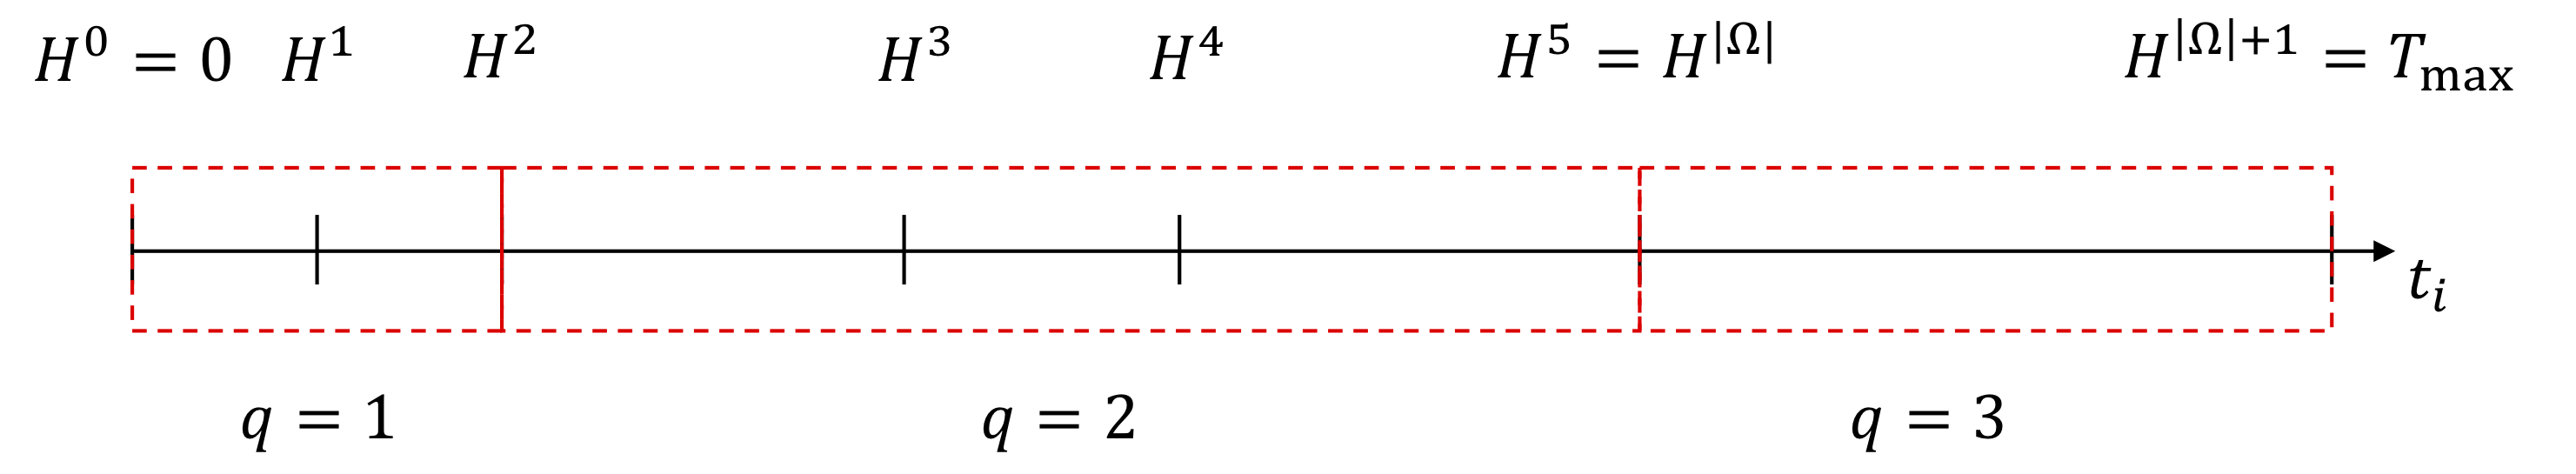
\includegraphics[width=0.8\textwidth]{simplePart}
		\caption{An illustration of a partition of interval \([0,T_{\max}]\)}
		\label{fig:simplePart}
	\end{figure}
	
	For each activity \(i \in I\) the first-stage start time \(t_i\) lies an interval of \(\cP_i\), and we introduce a first-stage indicator variable:
%	\begin{equation}
%		y_i^q = \begin{cases}
%			%1 & \text{if \(t_i \in [H^{\underbar{\omega}^q},H^{\bar{\omega}^q}]\)}\\
%			1 & \text{if \(t_i \in [\underbar{H}^q,\bar{H}^q]\)}\\
%			0 & \text{otherwise}
%		\end{cases}
%		\qquad \forall i \in I, q \in \cQ_i,
%	\end{equation}
%	and we use the following constraints to represent this relationship:
	\begin{subequations} \label{cons:yCons}
		\begin{align}
			& \sum_{q \in \cQ_i} \underbar{H}^q y_i^{q} \leq t_i \leq \sum_{q \in \cQ_i} \bar{H}^q y_i^{q} \qquad \qquad \forall i \in I \label{cons:tyBounds}\\
			& \sum_{q \in \cQ_i} y_i^q = 1 \qquad \qquad \forall i \in I \label{cons:sumy1} \\
			& y_i^q \in \{0,1\}, \quad \quad \forall i \in I, q \in \cQ_i.
		\end{align}
	\end{subequations}
	{Constraints~\eqref{cons:yCons} require that \(t_i\) be associated with one of the intervals of the partition. In model~\eqref{prob:extensive} if $t_i=H^\omega$ then $G_i^\omega$ can either be 0 (activity $i$ is said to start before $\omega$'s disruption) or 1 ($i$ starts after the disruption). If $t_i=\bar{H}^q = \underbar{H}^{q + 1}=H^\omega$ for some $\omega$ then the $y$-variables have a similar choice, and our convention is that if the $y$-variables choose $t_i \in [\underbar{H}^q,\bar{H}^q]$ then activity $i$ is said to start before the disruption and if $t_i \in [\underbar{H}^{q+1},\bar{H}^{q+1}]$ then $i$ starts after the disruption.}
%	\newline
	\subsection{Tightening Big-\(M\) with Partitions} \label{subsec:tightenM}
	 The tightness of ($S^\omega$)'s LP relaxation relies, in part, on the big-$M$ value used in constraints to represent the logical condition of whether activity \(i\) starts before or after a disruption. A smaller, but still valid, big-\(M\) value yields a tighter relaxation, and can further help prevent numerical issues~\citep[e.g.,][]{camm1990cutting,klotz2013practical}. We can rewrite constraints~\eqref{cons:sG1} and~\eqref{cons:sG2} as:
	\begin{equation} \label{cons:Grange}
	(\hat{t}_i - H^\omega)/M \leq G_i \leq (\hat{t}_i - H^\omega)/M + 1.
	\end{equation}
	Variable \(G_i\) can take a wider range of values when \(M\) is large. Tightening \(M\) hinges on specifying valid ranges for \(\hat{t}_i\). Furthermore, we know that if \(\hat{t}_i > H^{\omega'}\) for some \(\omega'\) then \(G_i\) has to take value 1 in all subproblems ($S^\omega$) with \(\omega < \omega'\). On the other hand, if \(\hat{t}_i < H^{\omega'}\) for some \(\omega'\) then \(G_i\) must be 0  for all subproblems ($S^\omega$) in which \(\omega > \omega'\). If we can fix the \(G_i\) for all \(i \in I\) to either 0 or 1 the resulting optimality cuts will be tight.
	
%	\newline
%    These observations inform us that a tighter \(M\) and more binary valued \(G\) can result from bounding the value of first stage variable \(t_i,\ \forall i \in I\). We start with a set of initial bounds specified by Proposition~\ref{prop:bounds}. From now on we assume the scenarios \(\omega \in \Omega\) are sorted according to their time \(H^\omega\) in an ascending order.
	%This means that suppose the optimal solution of model~\eqref{prob:extensive} is denoted as \((t^*,x^*,G^{*,\cdot},t^{*,\cdot},x^{*,\cdot})\), the latter two representing the scenario specific start time and crashing decisions, we have:
	{
	\begin{proposition} \label{prop:bounds}
		 Let \(t_i^0\) be the longest \(S\)-\(i\) path in the activity network \(\mathcal{G} = (I,\cA)\) in which the arc length of \((i,k) \in \cA\) is \(D_{ik}\) and in which no crashing is allowed. Let \(t^*\) denote (part of) an optimal solution to model~\eqref{prob:extensive}. Then there exists a \(t^*\) such that \(t^*_i \in [0,H^{|\Omega|} + t_i^0],\ \forall i \in I\) provided $M$ and $M_t$ are sufficiently large.
		 %\(T_{\max} = H^{|\Omega|} + t_T^0\), where 
	\end{proposition}
	\begin{proof}
		Constraint~\eqref{cons:nonnegt} enforces the lower bound of $0$.
		%under our assumption that $D_{ik} + d_{ik}^\omega \ge 0$ for all $(i,k) \in \cA$, $\omega \in \Omega$. \\
		By hypothesis \(t_k^0 - t_i^0 \geq D_{ik}, \forall (i,k) \in \cA\) since \(t_i^0\) is the longest \(S\)-\(i\) path of \(\mathcal{G}\) in which the arc length of \((i,k) \in \cA\) is \(D_{ik}\) and in which no crashing is allowed. We prove the upper bound on \(t_i^*\) by contradiction. 
		
		Suppose there does not exist a \(t^*\) such that \(t^*_i \in [0,H^{|\Omega|} + t_i^0],\ \forall i \in I\). Then for every \(t^*\), there must be a set \(I^* \subseteq I\) such that \(t_i^* > H^{|\Omega|} + t^0_i\) for $i \in I^*$. Let the corresponding optimal values of variables \(x_{ij}, G_i^\omega, t_i^\omega, x_{ij}^\omega, z_{ij}^\omega\) be denoted \(x_{ij}^*, G_i^{\omega,*}, t_i^{\omega,*}, x_{ij}^{\omega,*}, z_{ij}^{\omega,*}\), respectively. We can establish a feasible solution to model~\eqref{prob:extensive} as follows:
		\begin{subequations} \label{eqn:feasSol}
    		\begin{align}
    		    & \tilde{t}_i = H^{|\Omega|} + t^0_i \qquad \forall i \in I^* \label{eqn:tequal1} \\
    		    & \tilde{t}_i = t_i^* \qquad \forall i \in I \backslash I^* \label{eqn:tequal2}\\
    		    & \tilde{x}_{ij} = x_{ij}^* \qquad \forall i \in I, j \in J_i \\
    		    & \tilde{G}_i^\omega = G_i^{\omega,*} \qquad \forall i \in I, \omega \in \Omega \\
    		    & \tilde{t}_i^\omega = t^{\omega,*}_i \qquad \forall i \in I, \omega \in \Omega \\
    		    & \tilde{x}_{ij}^\omega = x_{ij}^{\omega,*} \qquad \forall i \in I, j \in J_i, \omega \in \Omega \\
    		    & \tilde{z}_{ij}^\omega = z_{ij}^{\omega,*} \qquad \forall i \in I, j \in J_i, \omega \in \Omega.
    		\end{align}
		\end{subequations}
		We see this solution is feasible by examining the constraints of model~\eqref{prob:extensive}:
		\begin{itemize}
		    % the separation constraints?
		    \item For constraint~\eqref{cons:Sep}, we examine the following four possible cases:
		    \begin{itemize}
		        \item \(i \in I^*, k \in I^*\): since \(\tilde{x}_{ij} \geq 0\) and \(t_k^0 - t_i^0 \geq D_{ik}\), we have \[\tilde{t}_k - \tilde{t}_i  = t_k^0 - t_i^0 \geq D_{ik} \geq D_{ik} \left(1 - \sum_{j \in J_i} e_{ij} \tilde{x}_{ij} \right);\]
		        \item \(i \in I^*, k \notin I^*\): we have \(\tilde{t}_i < t_i^*\) since \(i \in I^*\), and then \[\tilde{t}_k - \tilde{t}_i > t_k^* - t_i^* \geq D_{ik} \left( 1 - \sum_{j \in J_i} e_{ij} x^*_{ij} \right) = D_{ik} \left(1 - \sum_{j \in J_i} e_{ij} \tilde{x}_{ij} \right);\]
		        \item \(i \notin I^*, k \in I^*\): since \(t_i^* \leq H^{|\Omega|} + t_i^0\), \(\tilde{x}_{ij} \geq 0\) and \(t_k^0 - t_i^0 \geq D_{ik}\), we have
		        \[\tilde{t}_k - \tilde{t}_i = H^{|\Omega|} + t_k^0 - t_i^* \geq H^{|\Omega|} + t_k^0 - \left(H^{|\Omega|} + t_i^0 \right) = t_k^0 - t_i^0 \geq D_{ik} \geq D_{ik} \left (1 - \sum_{j \in J_i} e_{ij} \tilde{x}_{ij} \right ); \]
		        \item \(i,k \notin I^*\): the constraint is unchanged and feasible;
		    \end{itemize}
		    % can G_i^\omega remains the same?
		    \item For variable \(G_i^\omega\):
    		    \begin{itemize}
    		        \item if \(i \notin I^*\): we have \(\tilde{t}_i = t_i^*\). Therefore, constraints~\eqref{cons:G1}-\eqref{cons:tG2} is unchanged and feasible;
    		        \item if \(i \in I^*\): variable \(G_i^{*,\omega}\) is forced to take value \(1\) for all \(\omega \in \Omega\). Since \(\tilde{t}_i = H^{|\Omega|} + t_i^0 \geq H^{|\Omega|}\), for any \(\omega \in \Omega\), \(\tilde{G}_i^\omega = G_i^{*,\omega} = 1\) remains feasible. Therefore, constraints~\eqref{cons:G1}-\eqref{cons:tG2} hold for $M$ and $M_t$ sufficiently large.
    		    \end{itemize}
		    \item Since the values for \(\tilde{t}_i^\omega, \tilde{x}_{ij}, \tilde{x}_{ij}^\omega, G_i^\omega, z_{ij}^\omega\) all remain the same, constraints~\eqref{cons:Budget},~\eqref{cons:SingleBudget},~\eqref{cons:xG1}-\eqref{cons:Gbounds} are all satisfied by the solution in~\eqref{eqn:feasSol}.
		\end{itemize}
		We can also see that \(\tilde{t}_i \leq t_i^* ,\ \forall i \in I\) because of equations~\eqref{eqn:tequal1} and~\eqref{eqn:tequal2}. Thus, the feasible solution in~\eqref{eqn:feasSol} yields an objective function value \(p^0 \tilde{t}_T + \sum_{\omega \in \Omega} p^\omega \tilde{t}_T^{\omega} \le p^0 t_T^* + \sum_{\omega \in \Omega} p^\omega t_T^{*,\omega}\). This means that the feasible solution in~\eqref{eqn:feasSol} is optimal. As \(\tilde{t}_i \leq H^{|\Omega|} + t_i^0,\ \forall i \in I\), it contradicts the assumption that there does not exist an optimal solution with \(t^*_i \in [0,H^{|\Omega|} + t_i^0],\ \forall i \in I\). 
		%Suppose there exists some \(i\) such that \(t_i^* > T_{\max}\). Since activity \(T\) succeeds every activity in \(I\backslash\{T\}\), we have \(t_T^* > T_{\max}\). 
        %With $\tilde{G}_i^\omega=1$ for all $i \in I, \omega \in \Omega$ there is no coupling between variables $\tilde{t}_i^\omega$ and $\tilde{t}_i$. 
		%However, \(T_{\max}\) is also the objective function value obtained by the feasible solution in~\eqref{eqn:feasSol}, which contradicts that \(t^*\) is optimal. Therefore, for all activity \(i \in I\), \(t_i^*\) must be smaller or equal to \(T_{\max}\).
%		There, we can keep \(x^*\), \(G^{*,\omega}\), \(t^{*,\omega}\) and \(x^{*,\omega}\) for all \(\omega \in \Omega\) the same, and replace the \(t_i^*\) by \(\tilde{t}_i\) for all \(i \in \tilde{I}\) without violating any constraints. This yields another feasible solution which has a smaller value of \(t_T^*\) since \(T \in \tilde{I}, \tilde{t}_T = T_{\max} < t_T^*\). Therefore the new objective value obtained by this feasible solution is smaller, which contradicts the assumption that \((t^*,x^*,G^{*,\cdot},t^{*,\cdot},x^{*,\cdot})\) is an optimal solution.
		%\tcb{I think the statement of the proposition is correct, but I don't think the proof is valid. The objective function of model~\eqref{prob:extensive} is $p^0 t_T + \sum_{\omega \in \Omega} p^\omega t_T^\omega$. Your proof is making an argument based on $t_T^*$ being the objective function value rather than the {\em expected} duration. The $d_{ik}^\omega$ values can be negative and so the expected duration isn't $T_{\max}$.}
	\end{proof}}
	\noi For simplicity of exposition, we use a uniform upper bound on every \(t_i\) for \(i \in I\) as \(T_{\max} = H^{|\Omega|} + t_T^0\). While Proposition~\ref{prop:bounds} bounds the start-time variables, \(t_i,\ \forall i \in I\), to the interval \([0,T_{\max}]\),
	%, precedence relationships between activities allow for further tightening of the bounds, and 
	the $y$-variables of~\eqref{cons:yCons} allow for tighter bounds.   
	%The benefit of setting up the \(y\) variables is to obtain tighter bounds for \(t_i\) than the generic bounds \([0,T_{\max}]\) in Proposition~\ref{prop:bounds}. 
	Given a partition for each activity and given a first-stage solution with \(\hat{y}_i^{q}, \forall i \in I, q \in \cQ_i \), we can replace 
	%the big-\(M\) in 
	constraints~\eqref{cons:sG1} and~\eqref{cons:sG2} with:
	%of the scenario with moderate \(M_i^{\omega,+}\) and \(M_i^{\omega,-}\) because introducing variables \(y\) gives us better bounds on \(t_i\):
%	\begin{subequations}
%		\begin{align}
%			& M_i^{\omega,+} = \sum_{q \in \cQ_i} \bar{H}^q \hat{y}_i^q - H^\omega\\
%			& M_i^{\omega,-} = H^\omega - \sum_{q \in \cQ_i} \underbar{H}^q \hat{y}_i^q,
%		\end{align}
%	\end{subequations}
%	and the constraints~\eqref{cons:sG1} and~\eqref{cons:sG2} become:
	\begin{subequations} \label{cons:newBoundsm}
		\begin{align}
			H^\omega + G_i \left(\sum_{q \in \cQ_i} \bar{H}^q \hat{y}_i^q - H^\omega \right) \geq \hat{t}_i \qquad \qquad \forall i \in I\\
			H^\omega - (1 - G_i) \left(H^\omega - \sum_{q \in \cQ_i} \underbar{H}^q \hat{y}_i^q \right) \leq \hat{t}_i \qquad \qquad \forall i \in I.
		\end{align}
	\end{subequations}
%	The multiplication of \(G_i \hat{y}_i^q\) makes the dual of subproblem no longer linear of \(y\). To fix this, since \(\hat{y}_i^q\) is binary and \(G_i\) for all \(i \in I, q \in \cQ_i\), we can 
In a first-stage solution, $\hat{y}_i^q=1$ for a specific $q$ satisfying $\underbar{H}^{q} \le \hat{t}_i \le \bar{H}^{q}$, and verifying the validity of constraints~\eqref{cons:newBoundsm} in replacing~\eqref{cons:sG1}-\eqref{cons:sG2} is straightforward by enumerating the cases \(H^\omega \in [\underbar{H}^{{q}},\bar{H}^{{q}}]\), \(H^\omega < \underbar{H}^{{q}}\), and \(H^\omega > \bar{H}^{{q}}\). In the degenerate case in which $H^\omega$ coincides with $\bar{H}^q$ or $\underbar{H}^q$, the corresponding constraint from~\eqref{cons:newBoundsm} is as tight as possible, i.e., a simple bound on $\hat{t}_i$ involving $H^\omega$. Otherwise constraints~\eqref{cons:newBoundsm} reduce to the following analog of~\eqref{cons:Grange}:
\begin{equation}
	(\hat{t}_i - H^\omega) / (\bar{H}^q-H^\omega) \leq G_i \leq  (\hat{t}_i - H^\omega)/(H^\omega-\underbar{H}^q) + 1,
\end{equation}
and we see that smaller values of $\bar{H}^q$ and larger values of $\underbar{H}^q$ have the effect of tightening the big-$M$ value in constraints~\eqref{cons:Grange}.
 

We introduce variables \(F_i^q\) to linearize the bilinear terms, and rewrite constraints~\eqref{cons:newBoundsm} as follows:
	\begin{subequations} \label{cons:newBoundsmlin}
		\begin{eqnarray}
			&&\sum_{q \in \cQ_i} \bar{H}^q F_i^q - H^\omega G_i \geq \hat{t}_i- H^\omega \qquad \qquad \forall i \in I \label{cons:FG1}\\
			&&H^\omega G_i  - \sum_{q \in \cQ_i} \underbar{H}^q F_i^q \leq \hat{t}_i - \sum_{q \in \cQ_i} \underbar{H}^q \hat{y}_i^q \qquad \qquad \forall i \in I \label{cons:FG2}\\
			&&F_i^q \leq G_i \qquad \qquad \forall i \in I, q \in \cQ_i \label{cons:FGlin1}\\
			&&F_i^q \leq \hat{y}_i^q \qquad \qquad \forall i \in I, q \in \cQ_i \label{cons:FGlin2}\\
			&&F_i^q \geq G_i + \hat{y}_i^q - 1 \qquad \qquad \forall i \in I, q \in \cQ_i. \label{cons:FGlin3}
		\end{eqnarray}
	\end{subequations}

\begin{comment}
	In the subproblem, for each activity \(i \in I\), there is only one \(\hat{q} \in \cQ_i\) such that \(\hat{y}_i^{\hat{q}} = 1\), which means \(\hat{t}_i \in 
	%[H^{\underbar{\omega}^{\hat{q}}},H^{\bar{\omega}^{\hat{q}}}]\). 
	[\underbar{H}^{\hat{q}},\bar{H}^{\hat{q}}]\). 
	We examine the validity and effectiveness result of these tightened constraints. For validity, we check if constraints~\eqref{cons:newBoundsm} matches the logic when \(G_i\) is binary, while for effectiveness, we need to compare the feasible range of \(G\) in constraints~\eqref{cons:Grange} and that specified by constraints~\eqref{cons:newBoundsm}.
	
	For a specific \(i \in I\), constraints~\eqref{cons:newBoundsm} can be rewritten using \(\hat{q}\):
	\begin{subequations} \label{cons:sGnew}
		\begin{align}
		%H^\omega + G_i \left( H^{\bar{\omega}^{\hat{q}}} - H^\omega \right) \geq \hat{t}_i \label{cons:sGnew1}\\
		%H^\omega - (1 - G_i) \left(H^\omega - H^{\underbar{\omega}^{\hat{q}}} \right) \leq \hat{t}_i. \label{cons:sGnew2}
		H^\omega + G_i \left( \bar{H}^{\hat{q}} - H^\omega \right) \geq \hat{t}_i \label{cons:sGnew1}\\
		H^\omega - (1 - G_i) \left(H^\omega - \underbar{H}^{\hat{q}} \right) \leq \hat{t}_i. \label{cons:sGnew2}
		\end{align}
	\end{subequations}
	For a scenario \(\omega \in \Omega\), there are three possible positions of \(H^\omega\) relative to this range with \(\hat{y}_i^{\hat{q}} = 1\): 
	%\(H^\omega \in [H^{\underbar{\omega}^{\hat{q}}},H^{\bar{\omega}^{\hat{q}}}]\), \(H^\omega < H^{\underbar{\omega}^{\hat{q}}}\), or \(H^\omega > H^{\bar{\omega}^{\hat{q}}}\). 
	\(H^\omega \in [\underbar{H}^{\hat{q}},\bar{H}^{\hat{q}}]\), \(H^\omega < \underbar{H}^{\hat{q}}\), or \(H^\omega > \bar{H}^{\hat{q}}\). 
	When \(G_i = 1\), the left-hand side of constraint~\eqref{cons:sGnew1} is \(\bar{H}^{\hat{q}}\) and the left-hand side of constraint~\eqref{cons:sGnew2} is \(H^\omega\). When \(G_i = 0\), the left-hand side of constraint~\eqref{cons:sGnew1} is \(H^\omega\), and the left-hand side of constraint~\eqref{cons:sGnew2} is 
	%\(H^{\underbar{\omega}^{\hat{q}}}\).
	\(\underbar{H}^{\hat{q}}\).
	\begin{enumerate}
		\item 
			\(H^\omega \in
			 %[H^{\underbar{\omega}^{\hat{q}}},H^{\bar{\omega}^{\hat{q}}}]\): 
			 [\underbar{H}^{\hat{q}},\bar{H}^{\hat{q}}]\): 
			 we can see that if \(\hat{t}_i \geq H^\omega\), by logic \(G_i\) should take value \(1\). Constraints~\eqref{cons:sGnew} match \(\hat{t}_i \geq H^\omega\) for \(G_i = 1\) and is violated for \(G_i = 0\). Similar validity results hold if \(\hat{t}_i < H^\omega\). In addition, the possible value \(G_i\) can take changes from the one shown in~\eqref{cons:Grange} to:
			\begin{equation}
			%\left(\hat{t}_i - H^\omega \right)/\left( H^{\bar{\omega}^{\hat{q}}} - H^\omega \right) \leq G_i \leq (\hat{t}_i - H^\omega)/\left(H^\omega - H^{\underbar{\omega}^{\hat{q}}} \right) + 1
			\left(\hat{t}_i - H^\omega \right)/\left( \bar{H}^{\hat{q}} - H^\omega \right) \leq G_i \leq (\hat{t}_i - H^\omega)/\left(H^\omega - \underbar{H}^{\hat{q}} \right) + 1 \label{cons:case1}
			\end{equation}
			Since the value of \(M\) decreases compared to constraints~\eqref{cons:Grange}, when \(\hat{t}_i \geq H^\omega\), the lower bound increases and upper bound is \(1\). When \(\hat{t}_i < H^\omega\), the upper bound decreases and the lower bound is \(0\). Therefore, the feasible range of \(G_i\) for each \(i \in I\) shrinks, the subproblem relaxation is tightened.
		\item 
			%\(H^\omega < H^{\underbar{\omega}^{\hat{q}}}\): 
			\(H^\omega < \underbar{H}^{\hat{q}}\): 
			we can see \(G_i = 1\) is feasible and \(G_i = 0\) violates constraint~\eqref{cons:sGnew1}. The possible value \(G_i\) can take becomes:
			\begin{subequations}
				\begin{align}
				%G_i \geq \left(\hat{t}_i - H^\omega \right)/\left( H^{\bar{\omega}^{\hat{q}}} - H^\omega \right)\\
				%G_i \geq (\hat{t}_i - H^\omega)/\left(H^\omega - H^{\underbar{\omega}^{\hat{q}}} \right) + 1.
				G_i \geq \left(\hat{t}_i - H^\omega \right)/\left( \bar{H}^{\hat{q}} - H^\omega \right) \label{cons:case2eqn1}\\
				G_i \geq (\hat{t}_i - H^\omega)/\left(H^\omega - \underbar{H}^{\hat{q}} \right) + 1. \label{cons:case2eqn2}
				\end{align}
			\end{subequations}
			Notice that the inequality~\eqref{cons:case2eqn2} is strictly weaker than~\eqref{cons:case2eqn1} because the right-hand side of~\eqref{cons:case2eqn2} is smaller than 0 while the right-hand side of~\eqref{cons:case2eqn1} is positive. Similar to Case 1, the lower bound increases compared to using a large \(M\) and the upper bound is \(1\), and we achieve a tightened relaxation.
		\item 
			%\(H^\omega > H^{\bar{\omega}^{\hat{q}}}\): 
			\(H^\omega > \bar{H}^{\hat{q}}\): 
			we can see \(G_i = 0\) is feasible and \(G_i = 1\) violates constraint~\eqref{cons:sGnew2}. The possible value \(G_i\) can take becomes:
			\begin{subequations}
				\begin{align}
				%G_i \leq \left(\hat{t}_i - H^\omega \right)/\left( H^{\bar{\omega}^{\hat{q}}} - H^\omega \right)\\
				%G_i \leq (\hat{t}_i - H^\omega)/\left(H^\omega - H^{\underbar{\omega}^{\hat{q}}} \right) + 1.
				G_i \leq \left(\hat{t}_i - H^\omega \right)/\left( \bar{H}^{\hat{q}} - H^\omega \right) \label{cons:case3eqn1}\\
				G_i \leq (\hat{t}_i - H^\omega)/\left(H^\omega - \underbar{H}^{\hat{q}} \right) + 1. \label{cons:case3eqn2}
				\end{align}
			\end{subequations}
			Notice that the inequality~\eqref{cons:case3eqn1} is always weaker than~\eqref{cons:case3eqn2} because the right-hand side of~\eqref{cons:case3eqn1} is greater than 1 while the right-hand side of~\eqref{cons:case3eqn2} is between 0 and 1. Similar to Case 1, the upper bound decreases compared to using a large \(M\) and the lower bound is \(0\), and we achieve a tightened relaxation.
	\end{enumerate}
	The tightened constraints~\eqref{cons:newBoundsm} is shown to have validity and effectiveness properties. 
\end{comment}	
	
%	However, for the latter two situations, 
	%\(H^\omega < H^{\underbar{\omega}^{\hat{q}}}\) and \(H^\omega > H^{\bar{\omega}^{\hat{q}}}\), 
%	\(H^\omega < \underbar{H}^{\hat{q}}\) and \(H^\omega > \bar{H}^{\hat{q}}\), 
%	\(G_i\) can still take fractional value. 
We can further tighten the formulation by adding two constraints involving \(y\) that cover cases when \(G_i\) can be fixed to \(0\) or \(1\). Again given a partition of each activity and a first-stage solution \(\hat{y}_i^q, \forall i \in I, q \in \cQ_i\), we have:
		\begin{equation}\label{cons:subyG}
			%\sum_{q \in \cQ_i, H^\omega \leq H^{\underbar{\omega}^q}} \hat{y}_i^q \leq G_i \leq 1 - \sum_{q \in \cQ_i, H^\omega \geq H^{\bar{\omega}^q}} \hat{y}_i^q \qquad \forall i \in I 
			\sum_{q \in \cQ_i, H^\omega {\leq} \underbar{H}^q} \hat{y}_i^q \leq G_i \leq 1 - \sum_{q \in \cQ_i, H^\omega {\geq} \bar{H}^q} \hat{y}_i^q \qquad \forall i \in I.
		\end{equation}
\tcr{
%Do one or the other or both of $H^\omega \leq \underbar{H}^q$ and $H^\omega \geq \bar{H}^q$ need to be {\em strict} inequalities?
%Imagine the case in which the interval is $\underbar{H}^q=\bar{H}^q=H^\omega$ then we're infeasible for $\omega$.
%If $t_i=H^\omega$ for some $i$ and $\omega$ then $G_i^\omega$ has a choice; i.e., it can choose to either declare activity $i$'s start time to be before or after the disruption. Suppose we have the finest necessary partition in place. The way that constraints~\eqref{cons:yCons} are written, the $y$-variables have the same choice. If $t_i=H^2$ then the $y$-variables can either choose to associate $t_i$ with interval $[H^1,H^2]$ or with interval $[H^2,H^3]$.  
}
{For the case in which \(H^\omega \in (\underbar{H}^q,\bar{H}^q)\) for the $q$ with $\hat{y}_i^q=1$, constraint~\eqref{cons:subyG} adds no restriction, but for the cases in which \(H^\omega \le \underbar{H}^q\) and \(H^\omega \ge \bar{H}^q\), $G_i$ is forced to $1$ and $0$, respectively.}
\begin{comment}
	Again we check the validity and the effectiveness result of constraints~\eqref{cons:subyG} for the three situations listed above:
	\begin{enumerate}
		\item 
			%\(H^\omega \in [H^{\underbar{\omega}^{\hat{q}}},H^{\bar{\omega}^{\hat{q}}}]\): 
			\(H^\omega \in [\underbar{H}^{\hat{q}},\bar{H}^{\hat{q}}]\): 
			the lower bound is \(0\) since \(y_i^q = 0\) for all elements of partition left of \(\hat{q}\), and the upper bound is \(1\) because \(y_i^q = 0\) for all elements of partition right of \(\hat{q}\). Therefore, \(0 \leq G_i \leq 1\) is valid.
		\item 
			%\(H^\omega < H^{\underbar{\omega}^{\hat{q}}}\): 
			\(H^\omega < \underbar{H}^{\hat{q}}\): 
			the lower bound is \(1\) since the summation term, 
			%\(\sum_{q \in \cQ_i, H^\omega \leq H^{\underbar{\omega}^q}} \hat{y}_i^q\), includes \(y_i^{\hat{q}}\), 
			\(\sum_{q \in \cQ_i, H^\omega \leq \underbar{H}^q} \hat{y}_i^q\), includes \(y_i^{\hat{q}}\), 
			which forces \(G_i = 1\). This matches the logic since \(\hat{t}_i \geq H^\omega\).
		\item 
			\(H^\omega > \bar{H}^{\hat{q}}\): the upper bound is \(1\) since the summation term, \(\sum_{q \in \cQ_i, H^\omega \geq \bar{H}^q} \hat{y}_i^q\), includes \(y_i^{\hat{q}}\), which forces \(G_i = 0\). This matches the logic since \(\hat{t}_i \leq H^\omega\).
	\end{enumerate}
\end{comment}	
	\subsection{Partition-based Decomposition Method} \label{subsec:partition}
	 % 
	 % As we refine the partition of \(t\)-space, we can generate tightened Benders' cuts to approximate the recourse function. 
	 % %, we can determine the value of \(G_i\) in many subproblems, which strengthens the Benders' cuts.\\
	 
	Our decomposition algorithm to solve model~\eqref{prob:extensive} iteratively partitions the continuous feasible region of the first-stage $t$-variables by introducing binary variables that facilitate tighter optimality cuts. With the addition of constraints~\eqref{cons:newBoundsmlin} and~\eqref{cons:subyG}, the tightened subproblem is: 
	\begin{subequations}
		\label{prob:subTightened}
		\begin{align}
		(S_{\cP}^\omega) \qquad f^\omega_{\cP}(\hat{t},\hat{x},\hat{y}) = \min \quad & t_T \\
		\text{s.t.} \quad & \sum_{q \in \cQ_i} \bar{H}^q F_i^q - H^\omega G_i \geq \hat{t}_i - H^\omega \qquad \qquad \forall i \in I \label{cons:sFG1t}\\
		& H^\omega G_i - \sum_{q \in \cQ_i} \underbar{H}^q F_i^q \leq \hat{t}_i - \sum_{q \in \cQ_i} \underbar{H}^q \hat{y}_i^q \qquad \qquad \forall i \in I \label{cons:sFG2t}\\
		& F_i^q \leq G_i \qquad \qquad \forall i \in I, q \in \cQ_i \label{cons:sFGlin1t}\\
		& F_i^q \leq \hat{y}_i^q \qquad \qquad \forall i \in I, q \in \cQ_i \label{cons:sFGlin2t}\\
		& F_i^q \geq G_i + \hat{y}_i^q - 1 \qquad \qquad \forall i \in I, q \in \cQ_i. \label{cons:sFGlin3t}\\
		& G_i \geq \sum_{q \in \cQ_i, H^\omega \leq \underbar{H}^q} \hat{y}_i^q \qquad \qquad \forall i \in I \label{cons:syG1t}\\
		& G_i \leq 1 - \sum_{q \in \cQ_i, H^\omega \geq \bar{H}^q} \hat{y}_i^q \qquad \qquad \forall i \in I \label{cons:syG2t}\\
	    & \text{constraints~\eqref{cons:stG1}-\eqref{cons:subzbounds}} \\
		& 0 \leq F_i^q \leq 1 \qquad \qquad \forall \,i \in I, q \in \cQ_i\\
		& 0 \leq G_i \leq 1. \qquad \qquad \forall \,i \in I. \label{cons:G01t}
		\end{align}
	\end{subequations}
	We express $(S_{\cP}^\omega)$ in LP relaxation form, excluding constraints~\eqref{cons:subInt}. Let $\ell$ denote the iteration of the decomposition algorithm, and $(\hat{t}^\ell,\hat{x}^\ell,\hat{y}^\ell)$ denote a given first-stage decision. We solve \((S_{\cP}^\omega)\) for each \(\omega \in \Omega\) and construct an optimality cut of the form:
	\begin{equation} \label{cons:cut}
		\theta^\omega \geq v^{\omega,\ell} + \sum_{i \in I} \pi_i^{\omega,\ell} (t_i - \hat{t}_i^{\ell}) + \sum_{i \in I} \sum_{j \in J_i} \lambda_{ij}^{\omega,\ell} (x_{ij} - \hat{x}_{ij}^{\ell}) + \sum_{i \in I} \sum_{q \in \cQ^{\ell}_i} {\gamma_{i}^{\omega,\ell,q}} \left( y_i^{q} - \hat{y}_i^{q,\ell} \right).
	\end{equation}
	Here, $\theta^\omega$ is a continuous decision variable that forms an outer-linearization of $f^\omega_{\cP}(t,x,y)$; parameter~$v^{\omega,\ell}$ is the optimal value of \((S_{\cP}^\omega)\) at $(\hat{t}^\ell,\hat{x}^\ell,\hat{y}^\ell)$; and, coefficients \(\pi,\lambda\) and \(\gamma\) are appropriate sums of dual variables from the LP relaxation---e.g., $\pi_i^{\omega,\ell}$ involves dual variables from constraints~\eqref{cons:stG1}-\eqref{cons:stG2} and~\eqref{cons:sFG1t}-\eqref{cons:sFG2t}.
	Since we solve a linear relaxation, \(\theta^\omega\) is a lower bound on \(f^\omega(\hat{t}^\ell,\hat{x}^\ell,\hat{y}^\ell)\). However, the cut needs to be modified once the partition is updated to maintain validity, and we assume that the update only refines the partition for each \(i \in I\):
	\begin{definition} \label{definition:refinement}
		For two partitions \(\cP^1_i\) and \(\cP^2_i\), indexed by \(\cQ^1_i\) and \(\cQ^2_i\), respectively, we say \(\cP^2_i\) is a {\em refinement} of \(\cP^1_i\) provided:
		\begin{equation*}
		\forall q^2 \in \cQ^2_i, \exists q^1 \in \cQ^1_i \text{ s.t. } \bar{H}^{q^1} \geq \bar{H}^{q^2} \text{ and } {\underbar{H}^{q^1} \leq \underbar{H}^{q^2}}.
		\end{equation*}
	\end{definition}
	\noi At the current iteration for each \(i \in I\), let the partition \(\cP_i\) be indexed by \(\cQ_i\), and assume this partition is formed from earlier partitions by a sequence of refinements satisfying Definition~\ref{definition:refinement}. We can then find a set of intervals in the current partition,  \(\cP_i\), whose union is the \(q\)-th interval in partition \(\cP^\ell_i\) from previous iteration \(\ell\). We index such a {\em descendant set} by \(\Delta_i(\ell,q)\). Cut~\eqref{cons:cut} can then be updated to the following form:
	\begin{align} \label{cons:updatedcut}
		& \theta^\omega \geq v^{\omega,\ell} + \sum_{i \in I} \pi_i^{\omega,\ell} (t_i - \hat{t}_i^{\ell}) + \sum_{i \in I} \sum_{j \in J_i} \lambda_{ij}^{\omega,\ell} (x_{ij} - \hat{x}_{ij}^{\ell}) + %\nonumber \\
		%& \qquad 
		\sum_{i \in I} \sum_{q \in \cQ^{\ell}_i} \gamma_{i}^{\omega,\ell,q} \left( \sum_{q^\prime \in \Delta_i(\ell,q)} y_i^{q^\prime} - \hat{y}_i^{q,\ell} \right). %\qquad \forall \ell = 1,2, \dots.
	\end{align}
	We show that given a partition, \(\cP=\bigtimes_{i \in I} \cP_i\), which is updated by sequential refinement from a previous partition, \(\cP^\ell = \bigtimes_{i \in I} \cP_i^\ell\), the optimality cut~\eqref{cons:updatedcut} is a valid lower approximation for~$f^\omega_{\cP}(t,x,y)$.
	\begin{proposition} \label{prop:validity}
		For each $i \in I$, suppose we have a partition, \(\cP_i\), indexed by \(\cQ_i\), which is a refinement of \(\cP_i^\ell\), indexed by \(\cQ_i^\ell\). Then at any given feasible \((t,x,y)\) we have
{
	\scalefont{0.950}		
		\begin{align} \label{cons:validlb}
			&f^\omega_{\cP}(t,x,y) \geq v^{\omega,\ell} + \sum_{i \in I} \pi_i^{\omega,\ell} (t_i - \hat{t}_i^{\ell}) + \sum_{i \in I} \sum_{j \in J_i} \lambda_{ij}^{\omega,\ell} (x_{ij} - \hat{x}_{ij}^{\ell}) + %\nonumber \\ 
			%& \qquad \qquad 
			\sum_{i \in I} \sum_{q \in \cQ^{\ell}_i} \gamma_{i}^{\omega,\ell,q} \left( \sum_{q^\prime \in \Delta_i(\ell,q)} y_i^{q^\prime} - \hat{y}_i^{q,\ell} \right). % \qquad \forall \ell = 1,2, \dots. 
		\end{align}
}
	\end{proposition}
	\begin{proof}
		We denote the recourse function corresponding to partition \(\cP^{\ell}\) by \(f^\omega_{\cP^\ell}(t,x,y)\), where \(y\) has the correct dimension according to \(\cP^\ell\). We first show that 
		\begin{equation} \label{cons:gglb}
			f^\omega_{\cP}(t,x,y) \geq f^{\omega}_{\cP^\ell}(t,x,\tilde{y}),
		\end{equation}
		where 
		\begin{equation}\label{eqn:y_ytilde_sub}
		    \tilde{y}_i^{q} =  \sum_{q^\prime \in \Delta_i(\ell,q)} y_i^{q^\prime} \qquad  \forall i \in I, q \in \cQ^\ell_i.
		 \end{equation}
		Suppose for given \((t,x,y)\), we solve (\(S_{\cP}^\omega\)) and obtain an optimal solution \((t^{\omega},x^{\omega},G^{\omega},F^{\omega})\). We then form \[\tilde{F}^{\omega,q}_i = \sum_{q^\prime \in \Delta_i(\ell,q) }F_i^{\omega,q^\prime} \qquad  \forall i \in I, q \in \cQ^\ell_i, \]
		and we obtain a feasible solution \((t^{\omega},x^{\omega},G^{\omega},\tilde{F}^{\omega})\) to subproblem (\(S_{\cP^\ell}^\omega\)). Therefore, inequality~\eqref{cons:gglb} holds. Furthermore, the cut generated under partition \(\cP^\ell\) is
		\[\theta^\omega \geq v^{\omega,\ell} + \sum_{i \in I} \pi_i^{\omega,\ell} (t_i - \hat{t}_i^{\ell}) + \sum_{i \in I} \sum_{j \in J_i} \lambda_{ij}^{\omega,\ell} (x_{ij} - \hat{x}_{ij}^{\ell}) + \sum_{i \in I} \sum_{q \in \cQ^{\ell}_i} \gamma_{i}^{\omega,\ell,q} \left( y_i^{q} - \hat{y}_i^{q,\ell} \right),\]
		 which means that for any feasible \((t,x,\tilde{y})\), we have 
		 \begin{equation} \label{cons:validglb}
		 	f^\omega_{\cP^\ell}(t,x,\tilde{y}) \geq v^{\omega,\ell} + \sum_{i \in I} \pi_i^{\omega,\ell} (t_i - \hat{t}_i^{\ell}) + \sum_{i \in I} \sum_{j \in J_i} \lambda_{ij}^{\omega,\ell} (x_{ij} - \hat{x}_{ij}^{\ell}) + \sum_{i \in I} \sum_{q \in \cQ^{\ell}_i} \gamma_{i}^{\omega,\ell,q} \left( \tilde{y}_i^{q} - \hat{y}_i^{q,\ell} \right).
		 \end{equation}
		 Using equation~\eqref{eqn:y_ytilde_sub}, we replace \(\tilde{y}\) by \(y\), and combine inequalities~\eqref{cons:gglb} and~\eqref{cons:validglb} to obtain~\eqref{cons:validlb}.
	\end{proof}
	\noi Proposition~\ref{prop:validity} states that by properly modifying the \(y\)-variables in cuts generated under earlier partitions, the resulting cuts~\eqref{cons:updatedcut} are valid in the sense of providing a lower approximation on the LP relaxation of the recourse function. Therefore, we incorporate the modified cuts~\eqref{cons:updatedcut} in the following master problem, given a partition \(\cP\), which is indexed by \(\cQ\):
	\begin{subequations} \label{prob:masterTightened}
		\begin{align}
		(M_{\cP}) \quad z_{\cP}^* = \min \quad &p^0 t_T + \sum_{\omega \in \Omega} p^\omega \theta^{\omega}\\
		\text{s.t.} \quad & t_k - t_i \geq D_{ik} \left ( 1 - \sum_{j \in J_i} e_{ij} x_{ij} \right ) \qquad \qquad \forall (i,k) \in \cA \label{cons:MpSep}\\
		& \sum_{i \in I} \sum_{j \in J_i} b_{ij}x_{ij} \leq B  \label{cons:MpBudget}\\
		& \sum_{j \in J_i} x_{ij} \leq 1  \qquad \qquad \forall \,i \in I \label{cons:MpSingleBudget}\\
		& \sum_{q \in \cQ_i} \underbar{H}^{q} y_i^{q} \leq t_i \leq \sum_{q \in \cQ_i} \bar{H}^{q} y_i^{q} \qquad \qquad \forall i \in I \label{cons:which_interval_for_t} \\
		& \sum_{q \in \cQ_i} y^q_i = 1 \qquad \qquad \forall i \in I \label{cons:MpY1}\\
		& \theta^\omega \geq v^{\omega,\ell} + \sum_{i \in I} \pi_i^{\omega,\ell} (t_i - \hat{t}_i^{\ell}) + \sum_{i \in I} \sum_{j \in J_i} \lambda_{ij}^{\omega,\ell} (x_{ij} - \hat{x}_{ij}^{\ell}) \nonumber \\
		&\qquad + \sum_{i \in I} \sum_{q \in \cQ^{\ell}_i} \gamma_{i}^{\omega,\ell,q} \left( \sum_{q' \in \Delta_i(\ell,q)}y_i^{q'} - \hat{y}_i^{q,\ell} \right) \qquad  \forall \omega \in \Omega, \ell = 1, 2, \dots, L \label{cons:master_the_cuts} \\
		& y_i^q \in \{0,1\} \qquad \qquad \forall i \in I, q \in \cQ_i \label{cons:binary_y_variables} \\
		& t_i \geq 0 \qquad \qquad \forall \,i \in I\\
		& 0 \leq x_{ij} \leq 1 \qquad \qquad \forall \,i \in I, j \in J_i.
		\end{align}
	\end{subequations}
	As we refine the partitions, the generated cuts become tighter and we provide tighter lower bounds on model~\eqref{prob:extensive}'s optimal value. We refine the partition by selecting the interval of \(\cP_i\) for each activity \(i \in I\), where for some scenarios \(\omega \in \Omega\) with \(H^\omega \in [\underbar{H}^q,\bar{H}^q]\), \(G_i^\omega\) has a fractional value, and partition the interval {as we describe in further detail in Section~\ref{subsec:refine}}. The decomposition procedure is given in Algorithm~\ref{alg:Cut}. \\
	\begin{algorithm}[ht]
		\caption{Partition-based decomposition algorithm to solve model~\eqref{prob:extensive}}
		\label{alg:Cut}
		\begin{algorithmic}[1]
			\State Initialize cut iteration number \(\ell = 0\), lower bound \(LB = 0\), upper bound \(UB = +\infty\), initial partition \(\cP^\ell\) with its indexed set \(\cQ^\ell\), and tolerance parameters \( \epsilon \ge \delta \ge 0\);
			\While{\(\frac{UB - LB}{UB} > \epsilon\)} \label{alg:while_step}
			\State Solve \((M_{\cP})\) and obtain solution \(\hat{t}^{\ell}, \hat{x}^{\ell}, \hat{y}^{\ell}, \hat{\theta}^{\ell}\) and optimal value \(z_{\cP}^*\);
			\If{\(z_{\cP}^* > LB\)}
			\State Update \(LB = z_{\cP}^*\);
			\EndIf
			\State For each \(\omega \in \Omega\), solve \((S^\omega)\) and obtain \(f^{\omega}(\hat{t}^{\ell},\hat{x}^{\ell})\) and \(\hat{G}^\ell\); 
			\State Calculate \(\bar{z} = p^0 \hat{t}^\ell_T + \sum_{\omega \in \Omega} p^\omega f^{\omega}(\hat{t}^\ell,\hat{x}^\ell)\); \label{alg:upper_bound_calculation} 
			\If{\(\bar{z} < UB\)} 
			\State Update \(UB =\bar{z}\) and incumbent solution as \(t^* = \hat{t}^\ell, x^* = \hat{x}^\ell\) and \(G^* = \hat{G}^\ell\);
			\EndIf
			\For{each \(\omega \in \Omega\)}
                \State solve \((S_{\cP}^\omega)\) given \(\hat{t}^{\ell}, \hat{x}^{\ell}, \hat{y}^{\ell}\) and obtain optimal value \(v^{\omega,\ell}\) and \(\pi^{\omega,\ell}, \lambda^{\omega,\ell}, \gamma^{\omega,\ell}\); \label{alg:step_to_solve_LP_sub}
                \If{\(\hat{\theta}^{\omega,\ell} < v^{\omega,\ell} - \delta\)}
                    add cut of form~\eqref{cons:cut} to \((M_{\cP})\);
                \EndIf
            \EndFor
            %\State Let \(\ell = \ell + 1\);
			%\State For each \(\omega \in \Omega\), 
			%\If{\(\bar{z}_{\cP} < p^0 \hat{t}^\ell_T + \sum_{\omega \in \Omega} p^\omega v^{\omega,\ell} - \delta\)}
			\If{there are cuts added}
			%\State Add \tcr{nonredundant} cuts of form~\eqref{cons:cut} to \((M_{\cP})\);
			\State Let \(\cP^{\ell + 1} = \cP^\ell\) and \(\cQ^{\ell + 1} = \cQ^\ell\); 
			\Else
			\State Refine the partition and obtain the new partition \(\cP^{\ell + 1}\) and its indexed sets \(\cQ^{\ell + 1}\); \label{alg:refine_partition}
			\State Update previously generated cuts to the form of~\eqref{cons:updatedcut};
			\EndIf
			\State Let \(\ell = \ell + 1\);
			\vspace{0.1cm}
			\EndWhile{\textbf{end while}}
			\State Output \(UB\) as the $\epsilon$-optimal value of model~\eqref{prob:extensive}, and \((t^*, x^*, G^*)\) as the $\epsilon$-optimal solution.
		\end{algorithmic}
	\end{algorithm}
	
%	\tcr{Do we need to make some assumption on $\delta$ relative to $\epsilon$? Suppose $\delta$ is huge; we'll never add a cut.}
	We prove Algorithm~\ref{alg:Cut} converges in finite number of iterations. Since every partition update is a refinement and we have a finite set of scenario \(\Omega\), we can prove the finite convergence of Algorithm~\ref{alg:Cut} as long as with the finest partition we reach the optimum of problem~\eqref{prob:extensive}.
%	We let $\cH=\{H^\omega \, | \, \omega \in \Omega \}$ denote the set of (distinct) disruption times. When a specific disruption time has scenarios with multiple magnitudes we have $|\cH| < |\Omega|$. 
 
	\begin{proposition} \label{prop:finestPar}
	Assume that the realizations of $H^\omega$, $\omega \in \Omega$, are distinct. Assume that for each partition, \({\cP}_i\) indexed by $\cQ_i$, and for each $H^\omega$ we have $H^\omega=\bar{H}^q$ for some $q \in \cQ_i$, i.e., $|\cQ_i|=|\Omega|+1$ so that each partition is as fine as possible. Then 
    \begin{equation}\label{eqn:proposition_equivalent}
        z^* = \min_{(t,x,y) \in \mathbb{X}}\ p^0 t_T + \sum_{\omega \in \Omega} p^\omega f^\omega_{{\cP}}(t,x,y),
    \end{equation}
		where 
		\begin{equation*}
			\mathbb{X} = \left\{(t,x,y) \left| 
			\begin{aligned}
			& \text{constraints } \eqref{cons:MpSep}\mbox{-}\eqref{cons:MpY1}\\ 
			&y_i^q \in \{0,1\} \qquad \forall i \in I, q \in {\cQ}_i\\
			& t_i \geq 0 \qquad \forall i \in I\\
			& 0 \leq x_{ij} \leq 1 \qquad \forall i \in I, j \in J_i
			\end{aligned}
			\right. \right\}
		\end{equation*}
	and where $z^*$ is the optimal value of model~\eqref{prob:extensive}.
	\end{proposition}
	\begin{proof}
        We can formulate an extensive form for model~\eqref{eqn:proposition_equivalent}, i.e., an analog of model~\eqref{prob:extensive}, using $\mathbb{X}$ and model~\eqref{prob:subTightened}, where the decision variables of model~\eqref{prob:subTightened} are now also indexed by $\omega$. Let $\Omega=\{1,2,\ldots,|\Omega|\}$ so that the realizations of the disruption times are given by $H^1 < H^2 < \cdots < H^{|\Omega|}$. By Definition~\ref{definition:partition}, under the hypothesis of the proposition, the intervals of each partition are given by the finest partition, $[H^0,H^1], [H^1,H^2], \ldots, [H^{|\Omega|-1},H^{|\Omega|}], [H^{|\Omega|},H^{|\Omega|+1}]$, which we can index by $q=1,2,\ldots,|\Omega|,|\Omega|+1$, where $H^0=0$ and $H^{|\Omega|+1}=T_{\max}$. Under the assumed partition, constraints~\eqref{cons:syG1t}-\eqref{cons:syG2t} in the extensive form of~\eqref{eqn:proposition_equivalent} reduce to
        \begin{equation}\label{eqn:one_to_one_formula}
            \sum_{q=\omega+1}^{|\Omega|+1} y_i^{q} \le G_i^\omega \le 1 - \left ( \sum_{q=1}^\omega y_i^{q} \right ), \forall i \in I, \omega \in \Omega.
        \end{equation}
        Under this finest partition, there is a one-to-one mapping between the $G$- and $y$-variables under the binary restrictions imposed by models~\eqref{prob:extensive} and~\eqref{eqn:proposition_equivalent}. In particular,  
        \begin{equation}\label{eqn:one_to_one}
        y_i^q=1 \ \mbox{if and only if} \  G_i^\omega=1 \  \forall \omega \ge q+1 \ \mbox{and} \ G_i^\omega=0 \ \forall \omega \le q. 
        \end{equation}
        Any feasible solution to model~\eqref{prob:extensive} necessarily satisfies the condition $G_i^{\omega} \le G_i^{\omega+1}$ required by~\eqref{eqn:one_to_one} via constraint~\eqref{cons:G2}. And, constraints~\eqref{cons:MpY1} and~\eqref{cons:binary_y_variables} ensures the $0$-$0$ or $1$-$1$ nature of the left- and right-hand side of~\eqref{eqn:one_to_one_formula}. By Proposition~\ref{prop:bounds} we know $t_i \in [0,T_{\max}]$, and hence this restriction imposed by model~\eqref{eqn:proposition_equivalent} is nonbinding. As a result, model~\eqref{prob:extensive} and the extensive form of model~\eqref{eqn:proposition_equivalent} are equivalent and yield the same optimal value. 
    \end{proof}
%under $F_i^{q,\omega}=G_i^\omega y_i^q$. 
%%%%%%%%%%%%%%%%%%%%%%%%%%%%%%%%%%%%%%%%%%%%%%%%%%%%%%%%%%%%%%%
\begin{comment}
For a feasible solution $(t,x)$ to model~\eqref{eqn:proposition_equivalent} the additional $y$-variables associate each first-stage $t_i$ with an interval on $[0,T_{\max}]$, which is not restrictive by Proposition~\ref{prop:bounds}. Given $(t,x)$ 
	
 Models~\eqref{prob:extensive} and~\eqref{prob:masterOri} have the same optimal value. For a feasible solution $(t,x)$ to model~\eqref{prob:masterOri} the additional $y$-variables associate each first-stage $t_i$ with an interval on $[0,T_{\max}]$, which is not restrictive by Proposition~\ref{prop:bounds}. \tcr{Subproblem~\((S_\cP^\omega)\), which defines $f^\omega_{{\cP}}(t,x,y)$, is a partial linear relaxation of the constraints of model~\eqref{prob:extensive}.} \tcb{I'm not sure this is true. The model defining $f^\omega_{{\cP}}(t,x,y)$ takes $y$ as input, which could be the {\em wrong} choice given $(t,x)$.} So \(z^*_\cP \leq z^*\) is automatically true.\\
		\newline
		Next we prove that, given the partition in~\eqref{eqn:partition}, we can construct a feasible solution, \((t^*,x^*,G^*)\), to the extensive formulation~\eqref{prob:extensive} with the same objective value from the optimal solution, \((\hat{t},\hat{x},\hat{y})\), to the problem
		\[\min_{(t,x,y) \in \mathbb{X}}\ p^0 t_T + \sum_{\omega \in \Omega} p^\omega f^\omega_{\hat{\cP}}(t,x,y).\]
		Suppose for \(i \in I\), we denote the index of partition where \(y\) variable takes value \(1\) as \(q_i\). Since \(\bar{H}^q = \underbar{H}^{q + 1},\ \forall q \in \hat{\cQ}_i\), either \(q_i \in \{q \in \hat{\cQ}_i \mid H^\omega \leq \underbar{H}^q\}\) or \(q_i \in \{q \in \hat{\cQ}_i \mid H^\omega \geq \bar{H}^q\}\) is true. Thus, constraints~\eqref{cons:syG1t} and~\eqref{cons:syG2t} enforce that \(G_i\) in the problem \((S_{\hat{\cP}}^\omega)\) takes binary value because the right-hand side expressions of those two constraints must be \(0\) or \(1\) simultaneously. This means that although subproblems are linear programs, the integrality is implied. Therefore, when we obtain the optimal solution \(\hat{G}^\omega\) from solving problems \((S_{\hat{\cP}}^\omega)\) for each \(\omega \in \Omega\), solution \((\hat{t},\hat{x},\hat{G})\) will be feasible for the extensive formulation because \((\hat{t},\hat{x},\hat{y}) \in \mathbb{X}\) and \(G\) variables satisfy the constraints~\eqref{cons:stG1}-\eqref{cons:subH} and binary constraints. This result is equivalent to \(z_{\hat{\cP}}^* \geq z^*\). Combining the results above we conclude that \(z^* = \min_{(t,x,y) \in \mathbb{X}}\ p^0 t_T + \sum_{\omega \in \Omega} f^\omega_{\hat{\cP}}(t,x,y).\)
\end{comment}	
%%%%%%%%%%%%%%%%%%%%%%%%%%%%%%%%%%%%%%%%%%%%%%%%%%%%%%%%%%%%%%%
	\begin{theorem} \label{thm:converge}
		Assume that the realizations of $H^\omega$, $\omega \in \Omega$, are distinct, and assume that we obtain a dual extreme-point solution to subproblem~\((S_{\cP}^\omega)\) in step~\ref{alg:step_to_solve_LP_sub} of Algorithm~\ref{alg:Cut}. Then, the algorithm terminates in finite number of iterations to an $\epsilon$-optimal solution to model~\eqref{prob:extensive} for any \(\epsilon \ge 0\). 
	\end{theorem}
	\begin{proof}
	Let $z^*$ denote the optimal value of model~\eqref{prob:extensive} or equivalently model~\eqref{prob:masterOri}. The value of $UB$ in the algorithm is an upper bound on $z^*$ because $(\hat{t}^\ell,\hat{x}^\ell)$ is a feasible solution, and its objective function value in model~\eqref{prob:masterOri} is evaluated in step~\ref{alg:upper_bound_calculation} of the algorithm. The value of $LB$ in the algorithm is a lower bound on $z^*$ because: (i)~Proposition~\ref{prop:validity} ensures that the cuts~\eqref{cons:master_the_cuts} are an outer linearizations of $f_{\cP}(t,x,y)$; inequality~\eqref{cons:gglb} in the proof of Proposition~\ref{prop:validity} shows that $f_{\cP}$ becomes tighter as the partition is refined; and, Proposition~\ref{prop:finestPar} shows that the finest partition yields a model equivalent to  model~\eqref{prob:extensive}. Thus, if Algorithm~\ref{alg:Cut} terminates according to step~\ref{alg:while_step} then the current incumbent is an $\epsilon$-optimal solution.      
	
	
	For a fixed partition, $\cP$, Algorithm~\ref{alg:Cut} can only add a finite number of new cuts because each linear program~\((S_{\cP}^\omega)\) has a finite number of dual extreme points. After the final iteration in which new cuts are added, partition $\cP$ is refined in step~\ref{alg:refine_partition} of the algorithm. Because there are a finite number of scenarios the finest possible partition, if necessary, will be obtained in a finite number of iterations. From Proposition~\ref{prop:finestPar} we know that with the finest partition the solution to model~\eqref{eqn:proposition_equivalent} yields an optimal solution, and we will obtain the requisite cuts~\eqref{cons:master_the_cuts} so that models~\eqref{prob:masterTightened} and~\eqref{eqn:proposition_equivalent} are equivalent in a finite number of iterations. 
	%	\(\hat{\cP}\) where for each \(i \in I\), \(|\hat{\cQ}_i| = |\Omega|\) and \(\bar{H}^q = \underbar{H}^{q + 1},\ \forall q \in \hat{\cQ}_i\), solving the problem \(\min_{(t,x,y) \in \mathbb{X}}\ t_T + \sum_{\omega \in \Omega} f^\omega_{\hat{\cP}}(t,x,y)\) is equivalent to solving the extensive formulation. Since there are only finite number of scenarios, it takes finite number of steps of refinement to reach the finest partition. \\
%		\newline
%		For each subproblem, there is only a finite number of possible values of dual variables because each corresponds to one of the finitely many different bases. This means that, for any partition \(\cP\), the recourse function \(f^\omega_{\cP}\) can be represented by finitely many linear cuts. Therefore, in algorithm~\ref{alg:Cut}, only a finite number of cuts are added for a finite number of partitions before \(UB = z^*\) and \(LB = z^*_{\hat{\cP}}\) is achieved, a.k.a. \(\frac{UB - LB}{UB} = 0\).
	\end{proof}
	
	\subsection{Pruning Partitions Using Bound Tightening} \label{subsec:FBBT}
	Feasibility-based and optimization-based bound tightening schemes have been proved powerful in mixed-integer nonlinear programming to improve computational performance~\citep[e.g.,][]{belotti2012fbbt,coffrin2015strengthening,sundar2018OBBT}. A feasibility-based bound tightening (FBBT) process is suitable for our problem because the precedence relationships limit the start times of  activities. We solve the following linear programs to identify the lower and upper bounds on the first-stage start time of each activity: 
	\begin{subequations} \label{prob:btminmax}
		\begin{align}
		\min/\max \quad & t_i \\
		\text{s.t.} \quad & \text{constraints \eqref{cons:MSep}-\eqref{cons:Mxbounds}}\\
		& \underbar{t}_i \leq t_i \leq \bar{t}_i \qquad \forall i \in I.
		\end{align}
	\end{subequations}
	The bound tightening process starts with a set of initial bounds \(\underbar{t}_i = 0\) and \(\bar{t}_i = T_{\max}\) for each \(i \in I\). We solve model~\eqref{prob:btminmax} iteratively and update \(\bar{t}_i\) and \(\underbar{t}_i\) until the bounds converge for every \(i \in I\).
	
	We run FBBT at the beginning of our decomposition method to provide the initial partition~\(\cP^0\) to start Algorithm~\ref{alg:Cut}. If we can tighten the bounds of some activities, for example, by branch-and-bound or heuristics, we can run FBBT to tighten the bounds for all activities, which leads to a tighter formulation of the subproblems, \((S^{\omega}_{\cP})\), as further detailed in Section~\ref{subsec:bbpartition}.
	
	\subsection{Obtaining a Heuristic Upper Bound} \label{subsec:HUB}
	In our computation, we observe that it can take many iterations of Algorithm~\ref{alg:Cut} before we find a good feasible solution. When there is not a tight upper bound to use as a ``cutoff value,'' it takes an integer programming solver longer to solve model \((M_{\cP})\). On the other hand, we can quickly solve the extensive formulation~\eqref{prob:extensive} when the number of scenarios is small; e.g., \(|\Omega| = 20\). Solving such a model provides a feasible first-stage solution \((\hat{t},\hat{x})\), which can be used to generate an upper bound for the problem with the larger, original set of scenarios. Therefore, we can generate \(N\) small subsets of scenarios from the original scenario set, i.e., \(\Omega_n \subset \Omega,\ n = 1,2,\dots,N\), and solve model~\eqref{prob:extensive} with each of those subsets to generate candidate upper bounds, and select the one with the smallest expected project span under $\Omega$. 
	
	In generating \(\Omega_n\), we observe that it is beneficial to have diverse scenarios within each subset.
	%in a similar distribution as the original scenario set. 
	As above, we sort the scenarios by disruption time so $H^\omega < H^{\omega+1}$. For simplicity, suppose each subset has equal size so that \(N \cdot |\Omega_n| = |\Omega|, \ \forall n\). The \(n\)-th subset is then:
	\[\Omega_n = \{ \omega \, | \, \omega=n + (j - 1) \cdot |\Omega_n|,\ j = 1,2,\dots, N\}.\]
	In Section~\ref{sec:results} we compare the computational time of the decomposition method with and without initial upper bounds, and show the significant performance improvement by including the heuristic upper bound.
	
	\subsection{Magnanti-Wong Cut Generation} \label{subsec:MW}
	In a Benders' decomposition algorithm, linear programming subproblems can have multiple optimal dual solutions, which means that at a specific incumbent solution, there are multiple valid cuts that could be generated. \citet{magnanti1981accelerating} provide a method to select Pareto-optimal cuts, which cannot be dominated, 
	%in the relative interior of the feasible region of the master problem. It means that the generated Pareto-optimal cuts have a higher value when the integrality is relaxed, 
	and help tighten the LP relaxation of the master program.
	
	We apply a technique that pursues the same goal as~\citeauthor{magnanti1981accelerating} in order to tighten cuts at interior points of \((M_\cP)\). We record \((\hat{t},\hat{x})\) solutions from previous iterations, compute the corresponding \(\hat{y}\) for the current partition, and obtain the average, which we denote (\(t^0,x^0,y^0\)). We then solve the subproblems following the procedure of~\citet{magnanti1981accelerating}, using this average point as a proxy for the core point, i.e., a point on the relative interior of the LP relaxation of \((M_{\cP})\)'s feasible region. For each scenario \(\omega \in \Omega\), first we solve model~\eqref{prob:subTightened} with the current master solution  \((\hat{t},\hat{x},\hat{y})\) to obtain the optimal value, \(f^{\omega}_{\cP}(\hat{t},\hat{x},\hat{y})\). Next we need to find dual variables that ensure the dual objective value at \((\hat{t},\hat{x},\hat{y})\) is within a small tolerance of \(f^{\omega}_{\cP}(\hat{t},\hat{x},\hat{y})\) (e.g., \(\epsilon_{MW} = 10^{-5}\)), while maximizing the dual objective value at \((t^0,x^0,y^0)\). Let the following denote the dual of \((S^\omega_\cP)\) in compact form, suppressing dependence on $\omega$:
	\begin{subequations} \label{prob:subdual}
		\begin{align}
		f^{\omega}_{\cP}(\hat{t},\hat{x},\hat{y})=
		\max_{\pi,\lambda,\gamma,\eta} \quad & \pi^\top (\hat{t} + b_t) + \lambda^\top (\hat{x} + b_x) + \gamma^\top (\hat{y} + b_y) + \eta^\top b \\
		\text{s.t.} \quad & A^\top_{\pi} \pi + A^\top_{\lambda} \lambda + A^\top_{\gamma} \gamma + A^\top_{\eta} \eta \leq c.
		\end{align}
	\end{subequations}
	%; Appendix~\ref{appen:probdual} details the full version of model~\eqref{prob:subdual}.
	We solve the following to obtain Magnanti-Wong cut parameters, \({v}\), \(\pi\), \(\lambda\), and~\(\gamma\):
	\begin{subequations} \label{prob:subMW}
		\begin{align}
		{v} = \max_{\pi,\lambda,\gamma,\eta} \quad & \pi^\top (t^0 + b_t) + \lambda^\top (x^0 + b_x) + \gamma^\top (y^0 + b_y) + \eta^\top b  \\
		\text{s.t.} \quad & \pi^\top (\hat{t} + b_t) + \lambda^\top (\hat{x} + b_x) + \gamma^\top (\hat{y} + b_y) + \eta^\top b \geq (1 - \epsilon_{MW}) f^{\omega}_{\cP}(\hat{t},\hat{x},\hat{y}) \\
		& A^\top_{\pi} \pi + A^\top_{\lambda} \lambda + A^\top_{\gamma} \gamma + A^\top_{\eta} \eta \leq c.
		\end{align}
	\end{subequations}
	\noi Our average point, (\(t^0,x^0,y^0\)), may not be in the relative interior of the master problem's feasible region, e.g.,  if all solutions contributing to the average have a component of $y$ taking value zero or one. Although this means the resulting  cuts may not be Pareto-optimal, they may still  improve computational performance, 
	%as shown in Table~\ref{table:heuristics} 
	and we investigate this in Section~\ref{sec:results}.
	
	\subsection{Cut Selection}\label{subsec:cut_selection}
	Algorithm~\ref{alg:Cut} is a multi-cut version of Benders' decomposition procedure~\citep{birge1988multicut}.
	%,trukhanov2010adaptive,birge2011introduction
	A multi-cut scheme can converge in fewer iterations, but each iteration is typically more computationally expensive. The latter issue tends to exacerbate as the algorithm proceeds and cuts accumulate, particularly when the master problem is a mixed-integer program.
	
	As we discuss in the next section, when naively keeping all cuts, we see that the time required to solve the master problem can grow quickly as the algorithm proceeds. Therefore, we limit the number of cuts and only keep those that have been tight most recently at the end of each Benders' iteration. Refining a partition can yield many loose cuts. Therefore, keeping only a limited number of cuts eliminates unnecessary constraints, while still providing a valuable lower bound and reducing computational effort. %Detailed computational results showing this effectiveness of cut selection is presented in Table~\ref{table:time}.
	
	%\tcr{Saying that we only keep the tight cuts is probably not a good idea. This can (in simpler settings) provably lead to cycling, where you delete cuts, add the same cuts again, etc. So, I modified what we have above.}

	\subsection{Refining Partitions}\label{subsec:refine} 
	Here, we indicate how a partition is refined in step~\ref{alg:refine_partition} of Algorithm~\ref{alg:Cut}. 
	%There could be many rules to refine the partition. 
	The most significant contributor to the optimality gap is that variable \(G\) can take fractional values in the relaxed problem~\((S_{\cP}^\omega)\). For example, if \(d_{ik}^\omega \gg D_{ik}\) then \(G_i\) can take a fractional value far from optimal.
	%For example, \(G_i\) should take value \(1\) when activity \(i\) starts after the disruption, but solving LP relaxation may output an optimal \(G_i\) as close to 0. 
	This can significantly alter the duration between activity \(i\) and \(k\) (see constraint~\eqref{cons:subSep}) in the LP relaxation, and thus create a large gap between the relaxation and the original mixed-integer subproblem. Let \(N_p\) be a parameter that limits the number of new partitions for each activity \(i \in I\); we use $N_p=5$ in our subsequent computation, unless stated otherwise. Suppose subproblem \((S_\cP^\omega)\) has as part of its solution \({G}_i^\omega, i \in I \). 
	%when we branch on the scenario \(\hat{\omega}\), suppose  
	Then separately for each $i \in I$ our rule selects for partitioning up to \(N_p\) scenarios with the largest values of:
	\begin{align}\label{eqn:define_rho}
	    \rho_{i}^{{\omega}} = \begin{cases}
    	\max_{(i,k) \in \cA} d_{ik}^{{\omega}} {G}_i^\omega & \text{if } t_i < H^{{\omega}}\\
    	\max_{(i,k) \in \cA} d_{ik}^{{\omega}} (1 - {G}_i^\omega) & \text{if } t_i > H^{{\omega}}\\
    	\min\{\max_{(i,k) \in \cA} d_{ik}^{{\omega}} {G}_i^\omega, \max_{(i,k) \in \cA} d_{ik}^{{\omega}} (1 - {G}_i^\omega)\} & \text{if $t_i=H^{\omega}$.}
    	\end{cases}
	\end{align}
	
	\subsection{Branch-and-Cut Algorithm}\label{subsec:bbpartition}
	In Algorithm~\ref{alg:Cut} we iteratively refine the partition defining the $y$-variables, and each time we solve master~\eqref{prob:masterTightened} we must solve a mixed-integer linear program, which we do with a commercial solver.
	Algorithm~\ref{alg:Cut} is not a branch-and-cut~(B\&C) algorithm in that it does not adaptively generate different cuts at different parts of a branch-and-bound tree. As a potential improvement to Algorithm~\ref{alg:Cut}, we propose here a B\&C algorithm, which involves a branch-and-bound (B\&B) tree with nodes that we manage. The root node in our B\&B tree involves the original partition, and we solve that node using Benders' decomposition, which iteratively adds cuts to master~\eqref{prob:masterTightened} until the problem is solved for the fixed partition, as in Algorithm~\ref{alg:Cut}. In the B\&C algorithm we recursively branch on a continuous variable $t_i$ via $t_i \le H^\omega$ and $t_i \ge H^\omega$ for some $i$-$\omega$ pair. Rather than actually branching on the continuous $t$-variables, this branching is carried out using the partition $(\cP_i,\cQ_i)$ by fixing the corresponding subset of $y_i^q$-variables to zero. This helps manage both the number of binary variables and the number of optimality cuts in a master problem. Moreover, in our implementation we solve the nodes in our B\&B tree in parallel.  

	%Algorithm~\ref{alg:Cut} can be further enhanced by a branch-and-cut process, which helps reduce the number of binary variables added to the master and enables solving simpler integer programs in parallel. 
	%The branch-and-bound (B\&B) tree consists of nodes corresponding to master problem~\eqref{prob:masterTightened} with additional branching constraints. 
	%The root node starts with the initial partition. 
	%For each B\&B node, we perform the Benders' decomposition process until it converges. 
	The optimal value of a B\&B node provides a lower bound on the optimal value of~\eqref{prob:extensive}. We also continually update a global upper bound each time we obtain a feasible solution in a Benders' decomposition iteration. If the gap between a node's lower bound and the global upper bound is smaller than the tolerance, we mark the node as fathomed. If not, we branch as follows:
    \begin{subequations}\label{eqn:branch_rule}
    	\begin{eqnarray}
    	&& \mbox{select} \ \omega \in \mbox{argmax}_{\omega \in \Omega}  \left [ f^{{\omega}}(\hat{t},\hat{x}) - f^{{\omega}}_{\cP}(\hat{t},\hat{x},\hat{y}) \right ] \label{eqn:branchselo} \\
    		&& \mbox{select} \ i \in \mbox{argmax}_{i \in I} \left [ \rho_i^\omega \right ]. \label{eqn:branchseli}
    	\end{eqnarray}
    \end{subequations}	
    In~\eqref{eqn:branchselo} we select the scenario~\({\omega}\) with the largest relaxation gap. Then in~\eqref{eqn:branchseli} we select the activity with the largest \(\rho_{i}^{{\omega}}\) from equation~\eqref{eqn:define_rho}. This defines the $i$-$\omega$ pair for branching on $t_i \le H^\omega$ versus $t_i \ge H^\omega$ using the $y$-variables in a form of SOS branching.
	%subproblem of scenario \(\hat{\omega}\) has a fractional \(G_i\).
%	The current node branches out to two children nodes: one with the constraint \(t_{\hat{i}} \leq H^{\hat{\omega}}\) and the other with the constraint \(t_{\hat{i}} \geq H^{\hat{\omega}}\). Correspondingly, the partition \(\cQ_{\hat{i}}\) will be refined because branching creates a natural partition at \(H^{\hat{\omega}}\), and some \(y_{\hat{i}}^{q}\) for the new partition will be forced to take value 0.\\
	
	After a branch, for each child node we refine the partition on all activities \(i \in I\) according to Section~\ref{subsec:refine}.
	%similar to the description in Section~\ref{subsec:partition}. 
	The children inherit the parent node's cuts, updated in a similar fashion as inequality~\eqref{cons:updatedcut}. To set up notation for Algorithm~\ref{alg:CutBB}, suppose that for activity \(i \in I\) the current B\&B node, say node \(n\), has a partition \(\cP_i^n\) indexed by set \(\cQ_i^n\), and its parent node \(m\) has a partition \(\cP_i^m\) indexed by set \(\cQ_i^m\). Then, the cuts inherited from node \(m\) are updated for node \(n\) as:
	\begin{align}\label{cons:updatedcutBB}
		& \theta^\omega \geq v^{\omega,m,\ell} + \sum_{i \in I} \pi_i^{\omega,m,\ell} (t_i - \hat{t}_i^{\, m,\ell}) + \sum_{i \in I} \sum_{j \in J_i} \lambda_{ij}^{\omega,m,\ell} (x_{ij} - \hat{x}_{ij}^{m,\ell}) + \nonumber \\
		& \qquad \sum_{i \in I} \sum_{q \in \cQ^{m}_i} \gamma_{i}^{\omega,m,q} \left( \sum_{q^\prime \in \Delta^n_i(m,q)} y_i^{q^\prime} - \hat{y}_i^{q,m,\ell} \right) \qquad \forall \ell = 1,2, \dots, L.
	\end{align}
	Here, \(\Delta^n_i(m,q)\) represents the descendant set of the partition \(\cP_i^n\) refined from the \(q\)-th element in the partition \(\cP_i^m\). The cuts remain valid by Proposition~\ref{prop:validity} because the partitions in the child node refine those of the parent node. The parent node is marked as fathomed after a refinement, and we select the next available node with the smallest lower bound.  

	Putting all these pieces together, we summarize our partition-based branch-and-cut decomposition method in Algorithm~\ref{alg:CutBB}. As indicated above, in implementation we execute the algorithm's steps on each available node in parallel.
	\begin{algorithm}[ht]
		\caption{Partition-based branch-and-cut algorithm to solve model~\eqref{prob:extensive}}
		\label{alg:CutBB}
		\begin{algorithmic}[1]
			\State Initialize tolerance parameters \(\epsilon \geq \delta \geq 0\), and a global upper bound \(UB\). 
			\State Initialize the B\&B tree with node \(1\), with the following properties: cut iteration number \(\ell_1 = 1\), lower bound \(LB^1\), initial partition \(\cP^1\) with its indexed set \(\cQ^1\);
			\While{there exists an available node such that \(\frac{UB - LB^n}{UB} > \epsilon\)}
			\State Select available node \(n\) with smallest \(LB^n\);
			\State Append inherited cuts from parent of node \(n\) to master~\((M^n_{\cP})\) using~\eqref{cons:updatedcutBB};
			\Repeat
    			\State Solve \((M^n_{\cP})\) and obtain solution \(\hat{t}^{\, \ell^n}, \hat{x}^{\ell^n}, \hat{y}^{\ell^n}, \hat{\theta}^{\ell^n}\) and optimal value \(z_{\cP}^*\);
    			\If{\(z_{\cP}^* > LB^n\)}
    			\State Update \(LB^n = z_{\cP}^*\);
    			\EndIf
    			\State For each \(\omega \in \Omega\), solve problem \((S^\omega)\) and obtain \(f^{\omega}(\hat{t}^{\ell^n},\hat{x}^{\ell^n})\) and \(\hat{G}^{\ell^n}\);
    			\State Calculate \(\bar{z} = p^0 \hat{t}^{\, \ell^n}_T + \sum_{\omega \in \Omega} p^\omega f^{\omega}(\hat{t}^{\ell^n},\hat{x}^{\ell^n})\);
    			\If{\(\bar{z} < UB\)} 
    			\State Update \(UB = \bar{z}\) and incumbent solution as \(t^* = \hat{t}^{\, \ell^n}, x^* = \hat{x}^{\ell^n}\) and \(G^* = \hat{G}^{\ell^n}\);
    			\EndIf
    			\For{each \(\omega \in \Omega\)}
                    \State solve \((S_{\cP}^\omega)\) given \(\hat{t}^{\, \ell^n}, \hat{x}^{\ell^n}, \hat{y}^{\ell^n}\) and obtain optimal value \(v^{\omega,\ell^n}\) and \(\pi^{\omega,\ell^n}, \lambda^{\omega,\ell^n}, \gamma^{\omega,\ell^n}\); \label{alg:bbCutLBSub}
                    \If{\(\hat{\theta}^{\omega,\ell} < v^{\omega,\ell} - \delta\)}
                        add cut of form~\eqref{cons:cut} to \((M^n_{\cP})\);
                    \EndIf
                \EndFor
    			\State Let \(\ell^n = \ell^n + 1\);
			\Until{no cut is added;}
			\If{\(\frac{UB - LB^n}{UB} > \epsilon\)}
			    \State Branch via~\eqref{eqn:branch_rule}, creating two available children nodes, \(n_1\) and \(n_2\), from node \(n\);
 %   			    \hspace{1cm} and mark them available;
			    \State Refine the partition for nodes \(n_1\) and \(n_2\) to obtain \(\cP^{n_1}\) and \(\cP^{n_2}\), respectively;
			    \State Let \(LB^{n_1} = LB^{n_2} = LB^n\);
			\EndIf
			\State Mark node \(n\) as fathomed;
			\vspace{0.1cm}
			\EndWhile{\textbf{end while}}
			\State Output \(UB\) as the $\epsilon$-optimal value of model~\eqref{prob:extensive}, and \((t^*, x^*, G^*)\) as the \(\epsilon\)-optimal solution.
		\end{algorithmic}
	\end{algorithm}
	
	\subsection{Algorithm~\ref{alg:CutBB}: Numerical Example}\label{subsec:numeg}
	We illustrate Algorithm~\ref{alg:CutBB} on an example with $\epsilon=0$. We consider the network with five activities that accompany the source and terminal, as shown in Figure~\ref{fig:fiveAct}. 
	\begin{figure}[H]
		\centering
		\includegraphics[width=0.6\textwidth]{fiveAct}
		\caption{A five-activity serial network to illustrate Algorithm~\ref{alg:CutBB}}
		\label{fig:fiveAct}
	\end{figure}
	\noi Each of the five activities has unit duration, and can be crashed with a single option that decreases the duration by 90\% with one unit of resource consumption, i.e., \(e_{i1} = 0.9,\ \forall i \in I \setminus \{S, T\}\), and we let \(B = 2\). The probability of no disruption is \(p^0 = 0.2\), and the disruption can occur at four discrete time points, \(H^1 = 1,\ H^2 = 2,\ H^3 = 3,\ H^4 = 4\), with equal probability \(p^\omega = 0.2,\ \forall \omega \in \Omega = \{1,2,3,4\}\). The increase in duration under a disruption is \(d_i^\omega = 10\) for each activity-scenario pair. By Proposition~\ref{prop:bounds} we can bound the start time of each activity from above by \(T_{\max} = 9\). 
	
	Running the FBBT procedure of Section~\ref{subsec:FBBT} we obtain $\underbar{t}_1=0, \, \underbar{t}_2=0.1, \, \underbar{t}_3=0.2, \, \underbar{t}_4=1.2,\underbar{t}_5=2.2$, and $\underbar{t}_T=3.2$. Given these values, and the realizations of $H^\omega$, we initialize node 1 of Algorithm~\ref{alg:CutBB} with the following partition, which precludes certain intervals for activities 4, 5, and $T$:
	\begin{align*}
	    &\cP_1^1 = \{[0,9]\} \qquad \qquad \;\; \cQ_1^1 = \{1\}\\
	    &\cP_2^1 = \{[0,9]\} \qquad \qquad \;\; \cQ_2^1 = \{1\}\\
	    &\cP_3^1 = \{[0,9]\} \qquad \qquad \;\; \cQ_3^1 = \{1\}\\
	    &\cP_4^1 = \{[0,1],[1,9]\} \qquad  \cQ_4^1 = \{1,2\} \qquad y_4^1 = 0\\
	    &\cP_5^1 = \{[0,2],[2,9]\} \qquad  \cQ_5^1 = \{1,2\} \qquad y_5^1 = 0\\
	    &\cP_T^1 = \{[0,3],[3,9]\} \qquad  \cQ_T^1 = \{1,2\} \qquad y_T^1 = 0.
	\end{align*}
	Excecuting steps 6-18 of the algorithm, we solve node 1 with Benders' decomposition, converging to an optimal value of \(z^*_{\cP} = 4.072\), and in the process, we obtain an upper bound of \(UB = 6.607\). The optimal solution is:
	\begin{align*}
	    & \hat{t}_1 = 0 \qquad \qquad \hat{x}_{11} = 0\\
	    & \hat{t}_2 = 1 \qquad \qquad \hat{x}_{21} = 0.1124\\
	    & \hat{t}_3 = 1.899 \qquad \; \hat{x}_{31} = 0.1124\\
	    & \hat{t}_4 = 2.798 \qquad \; \hat{x}_{41} = 0.8892\\
	    & \hat{t}_5 = 2.997 \qquad \; \hat{x}_{51} = 0.8860 \\
	    & \hat{t}_T = 3.2.
	\end{align*}
	 At this solution, by equation~\eqref{eqn:branchselo} the largest relaxation gap is incurred at \({\omega} = 1\), 
	 %with a value \(8.75\). 
	 and equation~\eqref{eqn:branchseli} corresponds to activity~3, which has a fractional solution of \(G_3 = 0.125\) in subproblem~\((S^1_\cP)\). We branch on $i$-$\omega$ pair 3-1, creating two children, node~\(2\) and node~\(3\). Node 2 has an additional constraint, \(t_3 \geq H^1 = 1\) and node 3 has an additional constraint \(t_3 \leq H^1 = 1\). For each activity \(i\), we refine the partition by selecting the scenario with the largest nonzero \(\rho_i^\omega\) for \(\omega \in \Omega\), i.e., for simplicity we use $N_p=1$; see Section~\ref{subsec:refine}. If the largest \(\rho_i^\omega\) is zero for activity $i$, we do not refine that activity's partition. We again apply the ideas of Section~\ref{subsec:FBBT}, and solve a series of linear programs~\eqref{prob:btminmax} to tighten the bounds of starting times for nodes~2 and~3, accounting for their respective additional constraints \(t_3 \geq 1\) and \(t_3 \leq 1\). This refinement and bound-tightening process yields:
 	\begin{align*}
 	    & \text{Node 2:}\\
	    &\cP_1^2 = \{[0,9]\} \qquad \qquad \qquad \quad \cQ_1^2 = \{1\}\\
	    &\cP_2^2 = \{[0,9]\} \qquad \qquad \qquad \quad \cQ_2^2 = \{1\}\\
	    &\cP_3^2 = \{[0,1],[1,9]\} \qquad \qquad \;\; \cQ_3^2 = \{1,2\} \qquad \quad  y_3^1 = 0\\
	    &\cP_4^2 = \{[0,1],[1,2],[2,9]\} \qquad  \cQ_4^2 = \{1,2,3\} \qquad y_4^1 = 0\\
	    &\cP_5^2 = \{[0,2],[2,3],[3,9]\} \qquad  \cQ_5^2 = \{1,2,3\} \qquad y_5^1 = 0\\
	    &\cP_T^2 = \{[0,3],[3,4],[4,9]\} \qquad  \cQ_T^2 = \{1,2,3\} \qquad y_T^1 = 0
	\end{align*}
	\begin{align*}
 	    & \text{Node 3:}\\
	    &\cP_1^3 = \{[0,1],[1,9]\} \qquad \qquad \;\; \cQ_1^3 = \{1,2\} \qquad \quad y_1^2 = 0\\
	    &\cP_2^3 = \{[0,1],[1,9]\} \qquad \qquad \;\; \cQ_2^3 = \{1,2\} \qquad \quad y_2^2 = 0\\
	    &\cP_3^3 = \{[0,1],[1,9]\} \qquad \qquad \;\; \cQ_3^3 = \{1,2\} \qquad \quad y_3^2 = 0\\
	    &\cP_4^3 = \{[0,1],[1,2],[2,9]\} \qquad  \cQ_4^3 = \{1,2,3\} \qquad y_4^1 = 0\\
	    &\cP_5^3 = \{[0,2],[2,3],[3,9]\} \qquad  \cQ_5^3 = \{1,2,3\} \qquad y_5^1 = 0\\
	    &\cP_T^3 = \{[0,3],[3,4],[4,9]\} \qquad  \cQ_T^3 = \{1,2,3\} \qquad y_T^1 = 0.
	\end{align*}
	We fathom node 1 and nodes~2 and~3 inherit its cuts and lower bound. Breaking the tie arbitrarily, we select and then solve node~2 with Benders' decomposition and obtain an optimal value of $z^*_{\cP} = 6.111$. Node~2 then branches to nodes~4 and~5, which inherit the cuts and the lower bound from node~2. The upper bound value remains $UB=6.607$.

	Node 3 now has the smallest lower bound, 4.072, among unfathomed nodes, and yields an optimal value of $z^*_{\cP} = 6$ and optimal solution: 
	\begin{subequations} \label{eqn:optSol}
        	\begin{align}
        	    & \hat{t}_1 = 0 \qquad \qquad \hat{x}_{11} = 1\\
        	    & \hat{t}_2 = 0.1 \qquad \quad\; \hat{x}_{21} = \frac{1}{9}\\
        	    & \hat{t}_3 = 1 \qquad \qquad \hat{x}_{31} = 0\\
        	    & \hat{t}_4 = 2 \qquad \qquad \hat{x}_{41} = 0\\
        	    & \hat{t}_5 = 3 \qquad \qquad \hat{x}_{51} = \frac{8}{9}\\
        	    & \hat{t}_T = 3.2.
        	\end{align}
    	\end{subequations}
    In the process of solving node 3, we also obtain a tighter global upper bound of $UB=6$ associated with solution~\eqref{eqn:optSol}, and hence the optimality gap at node~3 is zero. Nodes~4 and~5 can now be fathomed because their lower bound of 6.111 exceeds $UB$. The algorithm terminates with the optimal solution in equation~\eqref{eqn:optSol}, and the corresponding \(G\)-variables indicate that activities 1, 2, and 3 start before disruption scenario \(1\), activity 4 starts before disruption scenario \(2\), and activity 5 starts before disruption scenario \(3\). The optimal objective function value is $6= {0.6 \cdot \left [ 3.2 \right]  + 0.2 \cdot \left [ 2+ 11 \cdot (1-0.9 \cdot 8/9)+11 \right ]  + 0.2 \cdot \left [ 3 +11\cdot (1-0.9 \cdot 8/9) \right ]}$. 

\section{Experimental Results} \label{sec:results}
\tcr{Read all the red comments to the end before doing anything.}

%	\textcolor{blue}{Test results:
%	\begin{itemize}
%		\item Describe the test examples: where do they come from, number of nodes, how are they generated.
%		\item Cite Sen's paper and describe the implementation.
%		\item Results.
%	\end{itemize}}
	In this section, we address the following questions with our computational results:
	\begin{enumerate}
		\item What is the value of model~\eqref{prob:extensive}, which takes account of randomness in both the timing and magnitude of a disruption? In other words, 
		%what are other alternative solutions that are easier to obtain but possibly inferior? 
		how does the quality of the solution to model~\eqref{prob:extensive} compare to those of simpler alternatives?
		\item How does the solution quality improve as the number of samples grows in a sample average approximation? 
		\item How do Algorithms~\ref{alg:Cut} and~\ref{alg:CutBB} perform versus solving the extensive formulation~\eqref{prob:extensive} using a state-of-the-art MIP solver? How effective are the computational enhancements of upper-bound generation, Magnanti-Wong cuts, and the cut-selection procedure from Sections~\ref{subsec:HUB}-\ref{subsec:cut_selection}?
	\end{enumerate}
	Section~\ref{subsec:testcases} introduces the PERT networks and probability distributions characterizing the disruptions for our test cases. In Section~\ref{subsec:value} we construct deterministic and semi-deterministic alternatives to model~\eqref{prob:extensive}, perform out-of-sample tests, and compare the quality of the resulting solutions to those of model~\eqref{prob:extensive}. We test how the sample size affects solution quality and requisite computational effort in Section~\ref{subsec:budget}. Finally, in Section~\ref{subsec:time} we compare the performance of Algorithms~\ref{alg:Cut} and~\ref{alg:CutBB} to solving extensive formulation directly.

	All tests are run on a server with 30 Intel Xeon cores at 3.1 GHz and 256 GB of RAM. For Algorithm~\ref{alg:CutBB}, each node is solved by 6 cores and we allow at most 5 nodes to be solved simultaneously so that the maximum number of cores used at any time is again 30. All models are constructed using version 0.18.0 of the JuMP package~\citep{DunningHuchetteLubin2017} on the Julia platform. All linear programs and mixed-integer programs are solved by Gurobi 8.01~\citep{gurobi2016} with the integer feasibility tolerance and the primal feasibility tolerance both set to \(10^{-8}\). In addition, we solve all problems using an optimality-gap tolerance of $10^{-2}$, including Algorithm~\ref{alg:CutBB}'s $\epsilon=10^{-2}$ as well as $\delta=10^{-4}$.
	
	\subsection{Test Cases Construction} \label{subsec:testcases}
	%	\textcolor{blue}{Where we find our tests:
	%		\begin{itemize}
	%			\item Plambeck paper: Case 11
	%			\item V42: Case 14
	%			\item Case 19 from Elmgrabhy
	%			\item Case 55 from Elmgrabhy
	%			\item Randomized network 35, 75, 100 nodes
	%			\item Plambeck paper: Case 110
	%	\end{itemize}}
	
	
	%Although it is easy to construct an activity network with randomly distributed disruption time and magnitude, not all instances constructed can well illustrate properties of our problem. Therefore, 
	We construct our test cases based on two activity networks from the literature, along with one we create from ``scratch'' and one we generate randomly. In particular, we use an activity network from~\citet{plambeck1996sample} with 11 activities, and % and the other with 110 activities. 
	one from~\citet{Elmaghraby77} with 19 activities. 
	 %and the other with 55 activities. 
	 We also manually create one activity network with 14 activities and randomly generate one network with 35 activities using the tool \emph{RanGen}~\citep{demeulemeester2003rangen}.
	 %and generate two random networks with 75 and 100 activities, respectively using \textcolor{blue}{RanGen toolbox}. 
	 In the following section, we use ``Case \(X\)" to denote the test case with \(X\) activities. Data for all four test cases are detailed in Appendix~\ref{appen:data}.
	
	For each test case, the timing of the disruption is a discrete random variable sampled from a lognormal distribution, which is commonly used to model failure times~\citep[e.g.,][]{crow1987lognormal,mullen1998lognormal}. The magnitude of the disruption for each activity follows an exponential distribution (which we again sample) whose parameter varies among the activities; the exponential distribution is widely used to model activity durations such as service times~\citep[e.g.,][]{ross1996stochastic}.
	%. The exponential distribution can best model the drastic change caused by a disruption.
	\subsection{Value of a Fully Stochastic Model} \label{subsec:value}
	We compare the quality of five solutions, one from solving model~\eqref{prob:extensive} and four from solving simpler alternatives, to investigate the value of modeling both the random timing and random magnitude of a disruption. First, we can obtain a solution by solving a deterministic model~\eqref{prob:static}, assuming no disruption occurs, i.e., $d^\omega=0$ (denoted ``DET"). Three semi-stochastic alternative models can be solved assuming: both the timing and magnitude of the disruption are deterministic at their expected values (denoted ``EXP"); the timing is random but magnitude is fixed at its expected value (denoted ``\(H\)Only"); and, the magnitude is random but timing is fixed at its expected value (denoted ``\(d\)Only"). Finally, we construct the fully stochastic model~\eqref{prob:extensive} in which both the timing and magnitude are random (denoted ``FULL"). We sample \(500\) scenarios to solve \(H\)Only, \(d\)Only, and FULL. Twenty batches of samples of size 5,000 are used to estimate an upper bound for each candidate solution. The upper bound point estimate for those five candidate solutions is shown in Figure~\ref{fig:value}, and the \(95\%\) confidence interval is shown in Table~\ref{table:value}. \tcr{20 batches of size 5000 for the UB. This is the same as simply using a sample size of 100,000. The point estimates are identical. The sample variance is calculated slightly differently, but is the same in expectation. Right?} \tcb{Yes, the point estimates should have an identical mean no matter how large the sample size is. 20 batches are used just to calculate the variance.} \tcr{But, the point is that the sample variance of the 100,000 points ought to be the same as the sample variance of the 20 batches of 5,000: $\mbox{var} \frac{1}{n} \sum_{i=1}^n X_i = \frac{1}{n} \mbox{var} X_1$.  and $\mbox{var} \frac{1}{\ell} \sum_{j=1}^{\ell} \bar{X}^j_m = \frac{1}{\ell} \mbox{var}  \bar{X}_m = \frac{1}{\ell} \frac{1}{m} \mbox{var} X_1$. So, if $n=$100,000 and $\ell=20$ and $m=$5,000 then it should be the same. In other words, you can compute sample variance of 100,000 points or sample variance of 20 sample means, and it's the same. So, why batch at all? (Here, I've put aside the dividing by $n$ versus $n-1$ in the sample variance calculation, which does create small differences.) For the paper, let's just leave it as you have it. You can delete all these comments.}
	
	%by plugging each of these solutions in the SAA problem with the original \(500\) samples, and we call this estimation, \(z^*\), as ``in-sample" since these samples are also used to obtain solutions. We also sample 20 batches of samples of \(|\Omega| = 5000\), and obtain the confidence interval of the upper bound estimation, \(\bar{z}\), by testing the solution on these batches. We present the comparison of different solutions of Case 11 in Figure~\ref{fig:value}.
	\begin{figure}
		\centering
		\includegraphics[width=0.8\textwidth]{graphValues}
		\caption{Comparison of quality of alternative solutions in which the optimal value of ``FULL'' is rescaled to 1.0}
		\label{fig:value}
	\end{figure}
	
	Figure~\ref{fig:value} scales the optimal value of each test problem, dividing by that of FULL, and shows that the solution quality can be poor without considering uncertainty in the timing of a disruption. DET's upper bound estimate is at least \(20\%\) larger than that of FULL for all test cases. The upper bound estimates of \(d\)Only and EXP are similar and at least \(10\%\) larger than that of FULL. For Case 14, the upper bound of \(H\)Only is \(20\%\) larger than that of FULL, and is closer to that of FULL for the other three cases.  That said, given the sample sizes, the computational effort to solve \(H\)Only and FULL are comparable. These test results suggest that the solution to the fully stochastic model can outperform solutions to simpler variants. In the remainder of this section, we restrict attention to the FULL model.
	
	%, since we need to include the same number of binary variables and same disruption magnitude brings symmetry issues. 
	\begin{table}[H]
		%\centering
		\resizebox{\linewidth}{!}{%
		\begin{tabular}{ c | l | l | l | l | l }
			\hline
			& \thead{DET} & \thead{EXP} & \thead{\(d\)Only} & \thead{\(H\)Only} & \multicolumn{1}{c}{FULL}\\ \hline
			Case 11	&	575.80 \(\pm\) 16.88	&	454.33 \(\pm\) 18.34		&	454.33 \(\pm\) 18.34	&	287.05 \(\pm\) 14.91  &	287.29 \(\pm\) 14.92	\\
            Case 14	&	3309.27 \(\pm\) 177.18	&	2878.65 \(\pm\) 176.70 &	2876.42 \(\pm\) 176.55	&	3098.05 \(\pm\) 133.06	&	2602.97 \(\pm\) 110.12	\\
            Case 19	&	426.09 \(\pm\) 10.09	&	389.61 \(\pm\) 7.88	&	388.77 \(\pm\) 8.43	&	355.29 \(\pm\) 7.14	&	356.42 \(\pm\) 5.86	\\
            Case 35	&	1353.80 \(\pm\) 21.11	&	1183.74 \(\pm\) 18.52	&	1188.93 \(\pm\) 19.53	&	1078.57 \(\pm\) 17.31	&	1068.29 \(\pm\) 17.47	\\
			\hline
		\end{tabular}}
		\caption{Compare optimal values from alternatives of the disruption model}
		\label{table:value}
	\end{table}
	%\noi To further test whether having a fully stochastic model is the best, we run a pair-wise \(t\)-test. The null hypothesis is that whether the difference between the upper bound generated by one alternative solution and that generated by the fully stochastic solution is less than 0. The pair-wise \(t\)-test rejects all null hypotheses, which shows that the difference between an alternative solution is significantly larger than the fully stochastic solution. 
	
	\subsection{Solution Quality versus Sample Size} \label{subsec:budget}
	We examine the quality of solutions obtained by solving SAA problems with different sample sizes. In expectation, the optimal value of an SAA problem provides a lower bound on $z^*$, the optimal value of the population problem, and in expectation evaluating a sample-mean objective function of an SAA solution using an independent sample provides an upper bound on $z^* \,$\citep{mak_etal_1999}. Both estimates approach~$z^*$ as the sample size grows large~\citep[e.g.,][]{shapiro2009lectures}. Of course, the computational effort to solve the corresponding SAA problem grows with the sample size. Understanding how the solution quality improves with sample size helps us obtain a high-quality solution without excessive computational effort. For each test case, we first solve \(20\) SAA instances of model~\eqref{prob:extensive}, with sample sizes of 10, 20, 50, 100, 200, and 500. \tcr{I would not call $|\Omega|$ a sample size if you can avoid it. $\Omega$ is the sample space for the population problem as opposed to that of the SAA problem. (I removed $|\Omega|$.) You can delete this comment.} For each solution, we obtain a point estimate of the upper bound using the same 5,000 samples. We also obtain 95\% confidence intervals associated with both upper- and lower-bound estimators for each sample size. We present the upper bound results in Table~\ref{table:budgetU}, the lower bound results in Table~\ref{table:budgetL}, and a visualization of the estimators in Figure~\ref{fig:budget}.
	
	\begin{table}[H]
		%\centering
		\resizebox{\linewidth}{!}{%
		\begin{tabular}{ c | l l l l l l }
			\hline
	Sample size		& \multicolumn{1}{c}{10} & \multicolumn{1}{c}{20} & \multicolumn{1}{c}{50} & \multicolumn{1}{c}{100} & \multicolumn{1}{c}{200} & \multicolumn{1}{c}{500}  \\ \hline
			Case 11	&	326.05	\(\pm\)	80.59	&	293.43	\(\pm\)	24.20	&	290.95	\(\pm\)	28.51	&	283.06	\(\pm\)	12.24	&	280.10	\(\pm\)	6.59	&	278.33	\(\pm\)	2.30	\\
            Case 14	&	3002.42	\(\pm\)	537.69	&	2942.09	\(\pm\)	778.43	&	2714.87	\(\pm\)	330.61	&	2645.71	\(\pm\)	100.15	&	2627.94	\(\pm\)	40.46	&	2626.90	\(\pm\)	39.51	\\
            Case 19	&	385.41	\(\pm\)	42.29	&	383.67	\(\pm\)	45.78	&	358.99	\(\pm\)	16.76	&	355.28	\(\pm\)	10.21	&	352.57	\(\pm\)	7.65	&	350.91	\(\pm\)	1.83	\\
            Case 35	&	1130.18	\(\pm\)	117.51	&	1102.57	\(\pm\)	45.66	&	1091.34	\(\pm\)	33.00	&	1080.23	\(\pm\)	21.86	&	1073.05	\(\pm\)	10.53	&	1070.08	\(\pm\)	5.20	\\
			\hline
		\end{tabular}}
		\caption{Upper bound point estimates, and 95\% confidence intervals, for SAA solutions with different sample sizes \tcr{I want to confirm: The confidence intervals are with respect to 20 replications. So, for a sample size of 10 you find 20 first-stage decisions. You compute the sample mean objective function value for 5000 samples. You use the same 5000 samples and compute the confidence interval over the 20 observations.}}
		\label{table:budgetU}
	\end{table}

	\begin{table}[H]
		%\centering
		\resizebox{\linewidth}{!}{%
		\begin{tabular}{ c | l l l l l l }
			\hline
	Sample size & \multicolumn{1}{c}{10} & \multicolumn{1}{c}{20} & \multicolumn{1}{c}{50} & \multicolumn{1}{c}{100} & \multicolumn{1}{c}{200} & \multicolumn{1}{c}{500}  \\ \hline
			Case 11	&	296.44	\(\pm\)	255.34	&	247.24	\(\pm\)	134.57	&	266.30	\(\pm\)	140.43	&	275.33	\(\pm\)	73.14	&	289.32	\(\pm\)	66.97	&	274.79	\(\pm\)	36.59	\\
            Case 14	&	1868.25	\(\pm\)	2152.85	&	1991.32	\(\pm\)	1273.90	&	2244.39	\(\pm\)	992.31	&	2310.86	\(\pm\)	688.76	&	2508.60	\(\pm\)	456.24	&	2477.13	\(\pm\)	275.11	\\
            Case 19	&	310.07	\(\pm\)	123.11	&	324.00	\(\pm\)	85.84	&	331.84	\(\pm\)	53.49	&	339.69	\(\pm\)	36.10	&	344.84	\(\pm\)	21.78	&	345.10	\(\pm\)	14.26	\\
            Case 35	&	1166.85	\(\pm\)	586.64	&	1107.83	\(\pm\)	282.44	&	1055.84	\(\pm\)	202.07	&	1036.82	\(\pm\)	120.40	&	1060.78	\(\pm\)	82.29	&	1065.76	\(\pm\)	54.10	\\
			\hline
		\end{tabular}}
		\caption{Lower bound point estimates, and 95\% confidence intervals, for SAA solutions with different sample sizes}
		\label{table:budgetL}
	\end{table}
	
	\begin{figure}[H]
		\centering
		\includegraphics[width=\textwidth]{graphBudgets}
		\caption{Confidence intervals, and point estimates, of the lower upper bounds for different sample sizes \tcr{Please edit the cropping of the plots so the $y$-axis label isn't cut-off.}}
		\label{fig:budget}
	\end{figure}
	
	From the two tables and Figure~\ref{fig:budget}, we can see the gap between the upper- and lower-bound estimators shrinks, and both estimators become less variable as the sample size grows. Improvements in the upper-bound estimators are small for sample sizes that exceed 100, and while improvements in lower-bound point estimates can appear larger (see Case 14) they are small relative to sampling error for such sample sizes.  
	
	\subsection{Computational Performance} \label{subsec:time}
	In this section we discuss the computational performance of our decomposition method with its various potential enhancements. As a benchmark, we compare the performance of Algorithms~\ref{alg:Cut} and~\ref{alg:CutBB} to direct solution of the extensive formulation~\eqref{prob:extensive} using a commercial solver. 
%We also present how effective the techniques introduced in Section~\ref{sec:decomposition} are in terms of accelerating the decomposition method. 
	
	We first show the quality of the heuristic upper bound described in Section~\ref{subsec:HUB}. We solve SAA instances with sample sizes of 100, 200, and 500, and in the notation of Section~\ref{subsec:HUB} we use $N= $ 10, 10, and 20 in these three instances, respectively. We compare the heuristic upper bound to the optimal value of the SAA instance. Moreover, for each case/sample-size pair, we replicate the procedure on 20 independent instances. These are the same 20 instances used for sample sizes of 100, 200, and 500 in Section~\ref{subsec:budget} for which Table~\ref{table:budgetL} reports average optimal values. Table~\ref{table:hub} shows the smallest gap, the average gap, and the largest gap, all as percentages, between the heuristic upper bound and the SAA optimal value across the 20 replications. The table also shows the average time required to compute the heuristic upper bound.
	
	\begin{table}[H]
		\centering		
		\begin{tabular}{ c | c | r r r | r}
			\hline
			\multirow{2}{*}{\(\quad\)} & \multirow{2}{*}{Sample size} & \multicolumn{3}{c |}{Gap (\%)} & \multirow{2}{*}{Average time (Sec).} \\
		    & & Smallest & Average & Largest &\\
			\hline
			\multirow{3}{*}{Case 11} & 100 & 0.01	& 0.50 	& 2.30 	& 5.6\\
			& 200 & 0.00	& 0.15	& 0.83	& 17.8\\
			& 500 & 0.00	& 0.07	& 0.37	& 67.5\\
			\hline
			\multirow{3}{*}{Case 14} & 100 & 1.34	& 6.02	& 16.14	& 7.7\\
			& 200 & 1.58	& 3.90 	& 8.91	& 30.4\\
			& 500 & 0.75	& 2.35	& 3.96	& 104.4\\
			\hline
			\multirow{3}{*}{Case 19} & 100 & 0.56	& 2.67	& 5.28	& 9.9\\
			& 200 & 0.05	& 0.99	& 2.03	& 37.2\\
			& 500 & 0.00	& 0.72	& 1.59	& 127.6\\
			\hline
			\multirow{3}{*}{Case 35} & 100 & 0.00	& 0.64	& 2.65	& 5.8\\
			& 200 & 0.08	& 0.46	& 1.30	& 25.7\\
			& 500 & 0.00	& 0.32	& 1.25	& 59.0\\
			\hline
		\end{tabular}
		\caption{Gap between the heuristic upper bound and optimal value for 20 SAA replications}
		\label{table:hub}
	\end{table}
	
	We see that the average upper bound gap exceeds 5\% only for Case 14 when the sample size is 100. Among all 240 SAA instances, there are only 15 for which the heuristic upper bound exceeds the optimal value by more than 5\%. We also observe that as the sample size grows, the heuristic upper bound's quality improves. 
	
	Table~\ref{table:heuristics} shows run-time results for finding a heuristic upper bound and generating Magnanti-Wong cuts \tcr{while using Algorithm~\ref{}}. For all test cases we use a sample size of 500. We use $N=20$ for the heuristic upper bound, and we retain all the generated cuts. In the table, ``UB" means that we only use the heuristic upper bound of Section~\ref{subsec:HUB} and generate regular Benders' cuts, and ``MW" means that we generate Magnanti-Wong cuts of Section~\ref{subsec:MW} without the benefit of the upper bound heuristic. We also show the computation time of using neither and using both techniques.
	
	\begin{table}[H]
		\centering		
		\begin{tabular}{ c | r r r r }
			\hline
			Run time (sec.) & Case 11 & Case 14 & Case 19 & Case 35 \\ \hline
			Neither & 178.9 & 3,573.8 & 4,499.5 & 160.2 \\
			UB & 103.2 & 3,003.7 & 2,899.9 & 20.0\\
			MW & 180.5 & 2,386.4 & 2,002.1 & 320.4\\
			Both & 151.6 & 2,342.4 & 1,411.5 & 40.1\\
			\hline
		\end{tabular}
		\caption{Run-time results for using the heuristic upper bound and Magnanti-Wong cuts \tcr{in Algorithm~\ref{}}}
		\label{table:heuristics}
	\end{table}
	
	\tcr{Is Table~\ref{table:heuristics} based on 20 replications? (Either way, we should say. If not, we need to clarify because the first results use 20 replications.) As I indicate above, I'm not sure whether this is for Algorithm~1? In any case, I'm also not sure why the run-time values in Table~\ref{table:heuristics} don't appear somewhere in the 500 row of Table~\ref{table:time}? This section is unclear (to me) on whether FBBT is always being used? And, what is the effect of FBBT?}
	
	Table~\ref{table:heuristics} shows that obtaining a heuristic upper bound can reduce computational effort; this occurs because the bound facilitates earlier fathoming of some nodes in the branch-and-bound tree when solving the master MIP. This outweighs the time required to compute the upper bound; see Table~\ref{table:hub}. Magnanti-Wong cuts are effective for Cases~14 and~19 but not for the other two cases, and the two techniques can have a synergistic effect (Case 14). 
%The effectiveness of such cuts may depend on the geometric nature of test cases, and it is valuable to investigate this phenomenon with more test cases in the future.
	
	Table~\ref{table:time} compares the run time of Algorithm~\ref{alg:Cut} (denoted A\ref{alg:Cut}), Algorithm~\ref{alg:CutBB} (denoted A\ref{alg:CutBB}), with and without the cut selection procedure (CS); \tcr{these results use both the heuristic upper bound and Magnanti-Wong cuts. FBBT?}. The table also shows the run-time for solving the extensive formulation~\eqref{prob:extensive} using Gurobi, also to a relative optimality tolerance of 0.01. 
%The computational time is presented in Table~\ref{table:time}, assuming all techniques in Section~\ref{subsec:FBBT}-\ref{subsec:MW} are employed.
	
	\begin{table}[ht]
		\centering		
		\begin{tabular}{ c | c | r r r r r }
			\hline
			\multirow{2}{*}{Run time (sec.)} & \multirow{2}{*}{Sample size} & \multicolumn{5}{c}{Methods} \\ \cline{3-7}
			& & A\ref{alg:Cut} & A\ref{alg:Cut}+CS & A\ref{alg:CutBB} & A\ref{alg:CutBB}+CS & Extensive  \\ \hline
			\multirow{4}{*}{Case 11} & 100 & 14.6 & 12.1 & 20.0 & 10.0 & 7.1 \\
			& 200 & 27.8 & 60.8 & 20.0 & 30.0 & 49.9\\
			& 500 & 445.8 & 407.4 & 145.1 & 163.2 & 1,634.3\\
			& 1,000 & 411.2 & 500.0 & 80.1 & 88.1 & 5,622.7\\
			\hline
			\multirow{4}{*}{Case 14} & 100 & 83.5 & 57.4 & 70.1 & 60.1 & 17.2 \\
			& 200 & 246.9 & 233.2 & 212.9 & 136.4 & 212.7 \\
			& 500 & 2,882.6 & 2,635.8 & 1,651.5 & 1,122.1 & 1,677.0 \\
			& 1,000 & 10,388.4 & 12,692.3 & 4,777.6 & 2,673.7 & 12,027.1 \\
			\hline
			\multirow{4}{*}{Case 19} & 100 & 335.6 & 190.4 & 112.6 & 80.1 & 82.4 \\
			& 200 & 412.2 & 337.0 & 552.6 & 270.4 & 383.8 \\
			& 500 & 2,732.1 & 2,434.2 & 1,008.4 & 830.8 & 3,960.4 \\
			& 1,000 & 18,251.8 & 14,811.1 & 13,995.4 & 3,623.8 & 44,537.3 \\
			\hline
			\multirow{4}{*}{Case 35} & 100 & 60.5 & 57.5 & 50.0 & 40.0 & 9.6 \\
			& 200 & 18.9 & 17.5 & 20.0 & 20.0 & 40.3 \\
			& 500 & 81.9 & 80.5 & 30.0 & 30.0 & 346.9 \\
			& 1,000 & 313.0 & 303.9 & 50.1 & 50.1 & 690.5 \\
			\hline
		\end{tabular}
		\caption{Computational performance with different sample sizes for decomposition methods and directly solving the extensive formulation using Gurobi}
		\label{table:time}
	\end{table}
	
	% decomposition works
	Table~\ref{table:time} shows that although directly solving the extensive formulation may be faster when the sample size is small, our decomposition algorithms tend to perform better as the sample size grows; the table's one exception is Algorithm~\ref{alg:Cut} for Case 14. 
	%The only exception is in Case 14 where Algorithm~\ref{alg:Cut} has a longer running time than solving the extensive formulation, no matter whether we select cuts or not. 
	The improved computational performance occurs because, while our decomposition methods must solve the master problem multiple times, the number of binary variables is significantly smaller than that of the extensive formulation. %Therefore, when the sample size is large, our decomposition methods can outperform direct solution.
	
	% algorithm 2 is better, why
	Algorithm~\ref{alg:CutBB} outperforms Algorithm~\ref{alg:Cut} when the sample size exceeds 500. When the sample size is large, Algorithm~\ref{alg:Cut} requires many master iterations to converge, and solving the mixed-integer master program becomes significantly harder. For Algorithm~\ref{alg:CutBB}, the time saved by processing nodes in parallel outweighs the slightly longer solving time at each node due to using fewer cores. Moreover, because of branching, each master problem at a node in the B\&B tree has a small number of binary variables in Algorithm~\ref{alg:CutBB}, which further accelerates the B\&C algorithm. 
	% cut selection is useful, especially in algorithm 2
    The results also show that selecting cuts can significantly improve the decomposition methods.  On the most difficult instances, applying the cut selection scheme yields larger improvements for Algorithm~\ref{alg:CutBB} than for Algorithm~\ref{alg:Cut}. 
	%\begin{figure}
	%	\centering
	%	\includegraphics[width=0.8\textwidth]{case11_time}
	%	\caption{Computational performance for different sample sizes.}
		% \(|\Omega| \in \{100, 200, 300, 400, 500,1000\}\
	%	\label{fig:time}
	%\end{figure}
	
	\tcr{I'm a bit worried about the following in the computational results: 1. We argue that a sample size of about 100 is large enough to obtain good solutions. 2. Then  we show that you don't need to decomposition algorithm in this case.  We might be able to modify the first result by assessing solution quality using common random numbers. We'd do this by solving an SAA of sample size 10, 20, 50, 100, 200, 500, 1000. Then, we'd use 20 batches and compute the upper and lower bounds using a sample size of 10, 20, 50, 100, 200, 500, 1000. I suspect the sampling errors will be significantly smaller than what you present in the LB and UB tables and hence there may be an argument for needing the larger sample sizes.}
	
\section{Conclusions} \label{sec:conclusions}
	We introduce the concept of a stochastic disruption in the context of a project crashing problem. We consider the case of a single disruption, and formulate the model as a two-stage stochastic mixed-integer program in which the timing of the stage, i.e., the disruption time, is random.  We use examples to illustrate properties of our problem that deviate from its deterministic counterpart, including the fact that it can be optimal to delay the start of an activity or crash a shorter-duration activity, even under proportional reduction. While, conceptually, the underlying problem involves continuous decision variables, we argue that the problem is NP-hard. In our two-stage stochastic mixed-integer program, second-stage binary variables capture the logic of the start time of an activity, relative to the disruption time. The resulting model is computationally challenging, but we propose a decomposition method which exploits the logical temporal relationship just mentioned, and sequentially partitions the feasible region of continuous first-stage decision variables to generate tighter cuts in a Benders' decomposition algorithm. The proposed method can significantly improve computational performance, especially as sample sizes grow large.
	
 The ideas in this paper can be extended in multiple ways. There may be opportunities to exploit network structure in tailoring the branch-and-cut algorithm that we have developed. The distribution governing the disruption time and, conditional on that time, the magnitude of the disruption may facilitate sampling strategies that reduce variance and improve solution quality. We have considered a model and algorithm that allow for at most one disruption, but handling a small number of disruptions	could be attractive. 
	
%\tcr{	There are multiple possible extensions of the results in this paper. First, there is still room to improve the computational performance of the decomposition method. More branching and refining rules can be tested for the best computational performance. In addition, it is worthwhile to inspect the network structures so that we can improve the quality of cuts or prune partitions. }
	
\section*{Acknowledgements}

\tcr{To add}

\tcr{In the references: Why does the Ross {\em Stochastic Processes} book have a huge number of authors? I changed it to just him but am leaving this note in case something else was intended.}

	
\bibliographystyle{plainnat}
\bibliography{PERT_Bib}

\pagebreak

\appendix
%%%%%%%%%%%%%%%%%%%%%%%%%%%%%%%%%%%%%%%%%%%%%%%%%%%%%%%%%%%%%%%%%%%%%%%%%%%%%%%%%%%%%
\begin{comment}
\section{Detailed Formulation of Model~\eqref{prob:subdual}} \label{appen:probdual}
    The detailed version of model~\eqref{prob:subdual} is presented as follows:
    \begin{subequations}
        \begin{align}
            \max \quad & \sum_{i \in I} \sum_{q \in \cQ_i} \left[
            \hat{y}_i^q \lambda_{F2,i}^q + (\hat{y}_i^q - 1) \lambda_{F3,i}^q + \hat{y}_i^q \underbar{H}_i^q \lambda_{H2,i} + \lambda_{\bar{F},i}^q \right] + &\nonumber \\
            & \sum_{i \in I} \left[(H^\omega - \hat{t}_i) \lambda_{H1,i} - \hat{t}_i \left(\lambda_{H2,i} + \lambda_{t1,i} + \lambda_{t2,i} \right) + \lambda_{xs,i} + \lambda_{\bar{G},i} \right] + &\nonumber \\
            & \sum_{i \in I} \sum_{j \in J_i} \left[\hat{x}_{ij} \left(\lambda_{x1,ij} + \lambda_{x2,ij} \right) + \lambda_{\bar{z},ij} + \lambda_{\bar{x},ij} + \lambda_{z3,ij}\right] + &\nonumber \\
            & \sum_{i \in I} \left[ \left(\sum_{q \in \cQ_i: H^\omega \leq \underbar{H}_i^q} \hat{y}_i^q \right) \lambda_{y1,i} + \left(\sum_{q \in \cQ_i: H^\omega \geq \bar{H}_i^q} \hat{y}_i^q \right) \lambda_{y2,i} \right] + &\nonumber \\
            & B \lambda_{B} + \sum_{(i,k) \in \cA} D_{ik} \lambda_{d,ik} &\\
            \st \quad & -\lambda_{t1,i} - \lambda_{t2,i} -\lambda_{t3,i} + \sum_{(i,k) \in \cA} \lambda_{d,ik} - \sum_{(k,i) \in \cA} \lambda_{d,ki} \geq 0 & \forall\, i \in I\backslash\{T\} \label{cons:dualt1}\\
            & 1 - \lambda_{t1,i} - \lambda_{t2,i} -\lambda_{t3,i} + \sum_{(i,k) \in \cA} \lambda_{d,ik} - \sum_{(k,i) \in \cA} \lambda_{d,ki} \geq 0 & i = T \label{cons:dualt2}\\
            & -\lambda_{x1,ij} -\lambda_{x2,ij} +\lambda_{z2,ij} + \lambda_{z3,ij} - b_{ij} \lambda_B - & \nonumber \\
            & \qquad \qquad \lambda_{xs,i} - \lambda_{\bar{x},ij} - \sum_{(i,k) \in \cA} D_{ik} e_{ij} \lambda_{d,ik} \geq 0 & \forall\, i \in I, j \in J_i \label{cons:dualx}\\
            & \sum_{q \in \cQ_i} \left(\lambda_{F1,i}^q + \lambda_{F3,i}^q \right) - H^\omega \left(\lambda_{H1,i} - \lambda_{H2,i} \right) - \lambda_{y1,i} - \lambda_{y2,i} - \lambda_{\bar{G},i} + & \nonumber \\ 
            & \qquad \qquad \sum_{(k,i) \in \cA} \lambda_{G,ki} - \sum_{(i,k) \in \cA} \lambda_{G,ik} - M_t \lambda_{t1,i} + M_t \lambda_{t2,i} + H^\omega \lambda_{t3,i} + & \nonumber \\
            & \qquad \qquad \sum_{j \in J_i} \left(-\lambda_{x1,ij} + \lambda_{x2,ij} + \lambda_{z1,ij} + \lambda_{z3,ij} \right) + \sum_{(i,k) \in \cA} d_{ik}^\omega \lambda_{d,ik} \geq 0 & \forall\, i \in I \label{cons:dualG}\\
            &-\lambda_{F1,i}^q - \lambda_{F2,i}^q - \lambda_{F3,i}^q + \bar{H}_i^q \lambda_{H1,i} - \underbar{H}_i^q \lambda_{H2,i} - \lambda_{\bar{F},i}^q \geq 0 & \forall \, i \in I, q \in \cQ_i \label{cons:dualF}\\
            &-\lambda_{z1,ij} - \lambda_{z2,ij} - \lambda_{z3,ij} - \sum_{(i,k) \in \cA} d_{ik}^\omega e_{ij} \lambda_{d,ik} - \lambda_{\bar{z},ij} \geq 0 & \forall \, i \in I, j \in J_i \label{cons:dualz}\\
            & \lambda_{H1,i},\lambda_{y2,i},\lambda_{t2,i}, \lambda_{xs,i},\lambda_{\bar{G},i} \leq 0 & \forall\, i\in I \\
            & \lambda_{x2,ij}, \lambda_{z1,ij}, \lambda_{z2,ij}, \lambda_{\bar{x},ij}, \lambda_{\bar{z},ij} \leq 0 & \forall\, i \in I, j \in J_i \\
            & \lambda_{F1,i}^q,\lambda_{F2,i}^q,\lambda_{\bar{F},i}^q \leq 0 & \forall\, i \in I, q \in \cQ_i\\
            & \lambda_{G,ik} \leq 0 & \forall\, (i,k) \in \cA \\
            & \lambda_B \leq 0 &\\
            & \lambda_{H2,i},\lambda_{y1,i},\lambda_{t1,i},\lambda_{t3,i} \geq 0 & \forall\, i\in I \\
            & \lambda_{x1,ij}, \lambda_{z3,ij} \geq 0 & \forall\, i \in I, j \in J_i \\
            & \lambda_{F1,i}^q \geq 0 & \forall\, i \in I, q \in \cQ_i\\
            & \lambda_{d,ik} \geq 0 & \forall\, (i,k) \in \cA .
        \end{align}
    \end{subequations}
    
    \noi The formulation above is an exact form of model~\eqref{prob:subdual}. In this formulation, \(\lambda_{H1}\) and \(\lambda_{H2}\) are the dual variables of tightened logic constraints~\eqref{cons:sFG1t} and~\eqref{cons:sFG2t}. We use \(\lambda_{F1}, \lambda_{F2}\) and \(\lambda_{F3}\) to represent the dual variables for the linearization constraints~\eqref{cons:sFGlin1t}-\eqref{cons:sFGlin3t} for the bilinear term \(\hat{y}_i^q G_i\), and \(\lambda_{z1}, \lambda_{z2}\) and \(\lambda_{z3}\) to represent the dual variables for the linearization constraints~\eqref{cons:sublinearize1}-\eqref{cons:sublinearize3} for the bilinear term \(G_{i} x_{ij}\). The dual variables for the \(G\)-tightening constraints~\eqref{cons:syG1t} and~\eqref{cons:syG2t} are denoted as \(\lambda_{y1}\) and \(\lambda_{y2}\). \\
    \newline
    We use the dual variables \(\lambda_{t1}, \lambda_{t2}\) and \(\lambda_{t3}\) to denote the dual variables for the constraints~\eqref{cons:stG1},~\eqref{cons:stG2} and~\eqref{cons:subH}, all related to the variable \(t\), while we use the dual variables \(\lambda_{x1}\) and \(\lambda_{x2}\) to denote the dual variables for the constraints~\eqref{cons:sxG1} and~\eqref{cons:sxG2}, both related to the variable \(x\). The duration constraint~\eqref{cons:subSep} has its dual variable denoted as \(\lambda_{d}\), the single activity crashing budget constraint~\eqref{cons:subBudget1} has its dual variable as \(\lambda_{xs}\), and the overall crashing budget constraint~\eqref{cons:subBudget} has its dual variable as \(\lambda_B\). Finally, we use \(\lambda_{\bar{x}}, \lambda_{\bar{G}}\) and \(\lambda_{\bar{F}}\) to represent the dual variables for the upper bound of variables \(x\), \(G\), and \(F\), respectively.\\
    \newline
    The constraints in the dual formulation corresponds to variables in the primal subproblem. Constraints~\eqref{cons:dualt1} and~\eqref{cons:dualt2} are for variable \(t\), and for the terminal activity \(i = T\) we need to include the primal objective function coefficient, 1. We establish constraints~\eqref{cons:dualx} for variable \(x\), constraints~\eqref{cons:dualG} for variable \(G\), constraints~\eqref{cons:dualF} for variable \(F\), and constraints~\eqref{cons:dualz} for variable \(z\). All dual variables have the correct signs matching the sense of corresponding primal constraints.
\end{comment}
%%%%%%%%%%%%%%%%%%%%%%%%%%%%%%%%%%%%%%%%%%%%%%%%%%%%%%%%%%%%%%%%%%%%%%%%%%%%%%%%%%%%%

\section{Test Cases Data} \label{appen:data}
    We present the data of four test cases here. For all test cases we assume there is only one possible crashing option for each activity. The option consumes 1 unit of resource and has the effectiveness parameter of \(e_{i1} = 0.5\) for all \(i \in I\). The nominal scenario probability is \(p^0 = 0.1\) and \(p^\omega = \frac{1 - p^0}{|\Omega|}\). The timing of the disruption follows a lognormal distribution with parameters \(\mu\) and \(\sigma\) where the mode is \(e^{\mu - \sigma^2}\). We also assume that the duration only depends on the predecessor, i.e., \(D_{ik} = D_i\) and \(d_{ik}^\omega = d_i^\omega\). All \(d_i\) follow an exponential distribution with a mean of \(\mu_i\). The value of \(D_i\) and \(\mu_i\) are shown in the following tables.
    \pagebreak
    \begin{itemize}
        \item Case 11: \(B = 3, \mu = \ln 6, \sigma = 0.5\)
            \begin{figure}[H]
    		    \centering
    		    \includegraphics[width=0.9\textwidth]{case11}
    		    \caption{Activity network of Case 11}
    		    \label{fig:case11}
	        \end{figure}
	        \begin{table}[H]
	            \centering		
        		\begin{tabular}{ c | l | l l c| l | l}
        		    \cline{1-3}\cline{5-7}
        			Activity & \(D_{i}\) & \(\mu_i\) & \(\qquad\)& Activity & \(D_{i}\) & \(\mu_i\) \\
        			\cline{1-3}\cline{5-7}
        			1 & 10 & \(10^{-5}\) & & 7 & 7.3 & 1\\ 
        			2 & 2 & \(4\) & & 8 & 4.9 & 50\\ 
        			3 & 10 & \(2\) & & 9 & 11.1 & 40\\ 
        			4 & 12 & \(30\) & & 10 & 3.5 & 40\\ 
        			5 & 3 & \(1500\) & & 11 & 9.9 & 5\\ 
        			6 & 10 & \(1\) & &  &  & \\ 
        			\cline{1-3}\cline{5-7}
        		\end{tabular}
        		\caption{Activity duration \(D_i\) and the mean of disruption magnitude \(\mu_i\) for Case 11}
        		\label{table:case11}
	        \end{table}
	        \pagebreak
        \item Case 14: \(B = 4, \mu = \ln 35, \sigma = 0.5\)
            \begin{figure}[H]
    		    \centering
    		    \includegraphics[width=0.9\textwidth]{case14}
    		    \caption{Activity network of Case 14}
    		    \label{fig:case14}
	        \end{figure}
	        \begin{table}[H]
	            \centering		
        		\begin{tabular}{ c | l | l l c| l | l}
        		    \cline{1-3}\cline{5-7}
        			Activity & \(D_{i}\) & \(\mu_i\) & \(\qquad\)& Activity & \(D_{i}\) & \(\mu_i\) \\
        			\cline{1-3}\cline{5-7}
        			1 & 5 & \(10^{-5}\) & & 8 & 49 & 4000\\ 
        			2 & 30 & \(5\) & & 9 & 40 & 4000\\ 
        			3 & 25 & \(40000\) & & 10 & 30 & 3000\\ 
        			4 & 20 & \(40000\) & & 11 & 45 & 4000\\ 
        			5 & 15 & \(1500\) & & 12 & 25 & 5\\ 
        			6 & 24 & \(20000\) & & 13 & 21 & 5 \\ 
        			7 & 30 & \(20000\) & & 14 & 5 & 5 \\ 
        			\cline{1-3}\cline{5-7}
        		\end{tabular}
        		\caption{Activity duration \(D_i\) and the mean of disruption magnitude \(\mu_i\) for Case 14}
        		\label{table:case14}
	        \end{table}
	        \pagebreak
        \item Case 19: \(B = 4, \mu = \ln 8, \sigma = 0.5\)
            \begin{figure}[H]
    		    \centering
    		    \includegraphics[width=0.9\textwidth]{case19}
    		    \caption{Activity network of Case 19}
    		    \label{fig:case19}
	        \end{figure}
	        \begin{table}[H]
	            \centering		
        		\begin{tabular}{ c | l | l l c| l | l}
        		    \cline{1-3}\cline{5-7}
        			Activity & \(D_{i}\) & \(\mu_i\) & \(\qquad\)& Activity & \(D_{i}\) & \(\mu_i\) \\
        			\cline{1-3}\cline{5-7}
        			1 & 5 & \(10\) & & 11 & 6 & 400\\ 
        			2 & 10 & \(100\) & & 12 & 4.5 & 300\\ 
        			3 & 18 & \(300\) & & 13 & 12 & 1000\\ 
        			4 & 35 & \(300\) & & 14 & 1.5 & 10\\ 
        			5 & 6 & \(50\) & & 15 & 2.1 & 200\\ 
        			6 & 6 & \(50\) & & 16 & 8.1 & 2 \\ 
        			7 & 2.5 & \(400\) & & 17 & 6.1 & 100 \\ 
        			8 & 8 & \(20\) & & 18 & 0.001 & 40 \\ 
        			9 & 10 & \(1000\) & & 19 & 0.001 & 300 \\ 
        			10 & 1 & \(50\) & & & & \\ 
        			\cline{1-3}\cline{5-7}
        		\end{tabular}
        		\caption{Activity duration \(D_i\) and the mean of disruption magnitude \(\mu_i\) for Case 19}
        		\label{table:case19}
	        \end{table}
	        \pagebreak
        \item Case 35: \(B = 8, \mu = \ln 4, \sigma = 0.3\)
            \begin{figure}[H]
    		    \centering
    		    \includegraphics[width=\textwidth]{case35}
    		    \caption{Activity network of Case 35}
    		    \label{fig:case35}
	        \end{figure}
	        \begin{table}[H]
	            \centering		
        		\begin{tabular}{ c | l | l l c| l | l}
        		    \cline{1-3}\cline{5-7}
        			Activity & \(D_{i}\) & \(\mu_i\) & \(\qquad\)& Activity & \(D_{i}\) & \(\mu_i\) \\
        			\cline{1-3}\cline{5-7}
        			1 & 9 & \(10\) & & 19 & 8 & 10\\ 
        			2 & 7 & \(40\) & & 20 & 8 & 500\\ 
        			3 & 3 & \(30\) & & 21 & 1 & 500\\ 
        			4 & 4 & \(100\) & & 22 & 5 & 500\\ 
        			5 & 6 & \(50\) & & 23 & 2 & 10\\ 
        			6 & 3 & \(10\) & & 24 & 7 & 10 \\ 
        			7 & 10 & \(10\) & & 25 & 1 & 300 \\ 
        			8 & 4 & \(20\) & & 26 & 4 & 400 \\ 
        			9 & 3 & \(10\) & & 27 & 3 & 200 \\ 
        			10 & 6 & \(1000\) & & 28 & 4 & 1000 \\ 
        			11 & 9 & \(10\) & & 29 & 10 & 300\\ 
        			12 & 8 & \(500\) & & 30 & 7 & 500\\ 
        			13 & 5 & \(200\) & & 31 & 2 & 200\\ 
        			14 & 2 & \(10\) & & 32 & 9 & 100\\ 
        			15 & 5 & \(400\) & & 33 & 7 & 100\\ 
        			16 & 2 & \(10\) & & 34 & 1 & 100 \\ 
        			17 & 10 & \(10\) & & 35 & 7 & 200 \\ 
        			18 & 4 & \(2000\) & & & & \\ 
        			\cline{1-3}\cline{5-7}
        		\end{tabular}
        		\caption{Activity duration \(D_i\) and the mean of disruption magnitude \(\mu_i\) for Case 35}
        		\label{table:case35}
	        \end{table}
    \end{itemize}
    
\end{document}